\documentclass{article}
\usepackage[utf8]{inputenc}
\usepackage[english,russian]{babel}
\usepackage{amsmath}
\usepackage{enumerate}
\usepackage[12pt]{extsizes}
\usepackage{xcolor,listings}
\usepackage[left=30mm, top=20mm, right=20mm, bottom=20mm, nohead, footskip=10mm]{geometry}


\usepackage[absolute,overlay]{textpos}
\usepackage{indentfirst}
\usepackage{float}
\restylefloat{table}
\usepackage{hyperref}
\usepackage{mathtext}
\usepackage{amsfonts}
\usepackage{amsthm}
\usepackage{tikz}
\usetikzlibrary{shapes,positioning,shadows,trees,automata,arrows.meta,shapes.geometric}
\usepackage{pgf-pie}
\usepackage{chngcntr}
\usepackage{pdfpages}
\usepackage{systeme}
\usepackage{multirow}
\usepackage{empheq}
\usepackage{subcaption}
\numberwithin{equation}{section}
\counterwithout{figure}{section}

\pagestyle{plain}

\definecolor{String}{RGB}{134, 179, 0}
\definecolor{KeyColor}{RGB}{160,0,102}


\captionsetup[lstlisting]{
	singlelinecheck=false,
	margin=3pt,
	font=,skip=5pt,
	font={bf}
}

\lstdefinestyle{style}{
	aboveskip=0pt,
	belowskip=10pt,
	showspaces=false,
	showstringspaces=false,
	basicstyle=\ttfamily\footnotesize,
	numbers=left,
	% texcl=true,
	breaklines=true,
	postbreak=\mbox{\textcolor{red}{$\hookrightarrow$}\space},
	keywordstyle=\color{KeyColor},
	identifierstyle=\color{black},
	numberstyle=\scriptsize,
	stringstyle=\color{String},
	commentstyle=\color{gray},
	frame=tb
}

\begin{document}
    \thispagestyle{empty}
	\begin{center}
		Санкт-Петербургский политехнический университет Петра Великого\\
		Институт прикладной математики и механики\\
		Кафедра <<Телематика (при ЦНИИ РТК)>>\\
		\vspace*{\fill}
		\textbf{\Large{КУРСОВАЯ РАБОТА}}\\
		\vspace{0.5cm}
        \large{по дисциплине <<Семинар по роботизированным системам>>\\}
        \large{на тему <<Муравьиный алгоритм и алгоритм коллективного распределения целей>>}\\
        \vspace{1cm}
        по направлению 02.04.01.02 <<Организация и управление суперкомпьютерными системами>>
	\end{center}
	\vspace{3cm}
	\begin{tabular} {l l l}
	\hspace{10cm} & Выполнил: & Титов А.И.\\
	& Проверил: & Моторин Д.Е.
	\end{tabular}
	\vspace*{\fill}
	\begin{center}
		Санкт-Петербург\\
		2019
    \end{center}
    \newpage


	\renewcommand\contentsname{Оглавление}
	\tableofcontents

	\newpage
	\addcontentsline{toc}{section}{ПОСТАНОВКА ЗАДАЧИ}
	\section*{ПОСТАНОВКА ЗАДАЧИ}

	Целью курсовой работы является реализация и исследование алгоритмов для построения оптимальных путей роботов до целей. Далее под роботом, для простоты, будет иметься в виду непосредственно начальная координата пути, а под целью, соответственно, конечная координата.

	Таким образом, требуется создать карту местности, на которой помещается набор роботов и набор целей, после чего каждому роботу оптимально назначить цель и построить путь до нее.

	Для этого требуется реализовать следующие алгоритмы:

    \begin{itemize}
        \item Алгоритм для процедурного построения реалистичной карты местности \cite{terrain};
        \item Алгоритм коллективного распределения целей \cite{plan};
        \item Алгоритм поиска пути \cite{path}.
	\end{itemize}

	Для генерации реалистичной карты среды выбран алгоритм Diamond-Square \cite{DS}. Алгоритм коллективного распределения целей описан в \cite{plan} в главе <<Алгоритм коллективного улучшения плана 3.7>> на стр. 102. Для вычисления пути от робота до цели рассматривается муравьиный алгоритм \cite{ant}.

	Выполняются следующие задачи для достижения цели:
	\begin{enumerate}
		\item Реализация алгоритма Diamond-Square;
		\item Реализация муравьиного алгоритма;
		\item Реализация алгоритма коллективного распределения целей;
		\item Исследования реализованного функционала.
	\end{enumerate}

	Реализация осуществляется на языке Python. Исследование реализованного функционала заключается в следующем:

	\begin{enumerate}
		\item Генерация 10 различных карт для каждого размера из: 25x25, 50x50, 100x100, 250x250, 500x500, 1000x1000;
		\item На каждой из сгенерированных карт создаются наборы роботов и, соответственно, цели к ним в численности: 5, 10, 20, 50 (наборов каждого размера для каждой карты тоже должно быть по 10, но из соображений производительности этот пункт опущен);
		\item Для заданных наборов распределяются цели по роботам;
		\item Для каждого построенного набора строятся графики, отображающие зависимость времени выполнения программы от размеров карт и численности роботов. (В изначальном задании указано построить график, содержащий все измеренные времена, но для наглядности графики строятся только для средних элементов измерений времени, а полную картину отражают таблицы в \hyperref[sec:time]{ПРИЛОЖЕНИЕ Б});
		\item Теоретическое исследование реализуемого функционала.
	\end{enumerate}

	\newpage
	\section{Описание алгоритмов}

		В данной главе представлен разбор теоретических принципов работы реализуемых алгоритмов.

		\subsection{Алгоритм Diamond-Square}

			В данной работе для процедурной генерации реалистичной карты местности используется алгоритм Diamond-Square\cite{DS}. Прочие применяемые алгоритмы описаны в \cite{terrain}.

			Алгоритм имеет ограничения на размеры получаемой карты высот - $(2^{n} + 1)\times(2^{n} + 1)$.

			\begin{figure}[H]
				\centering
				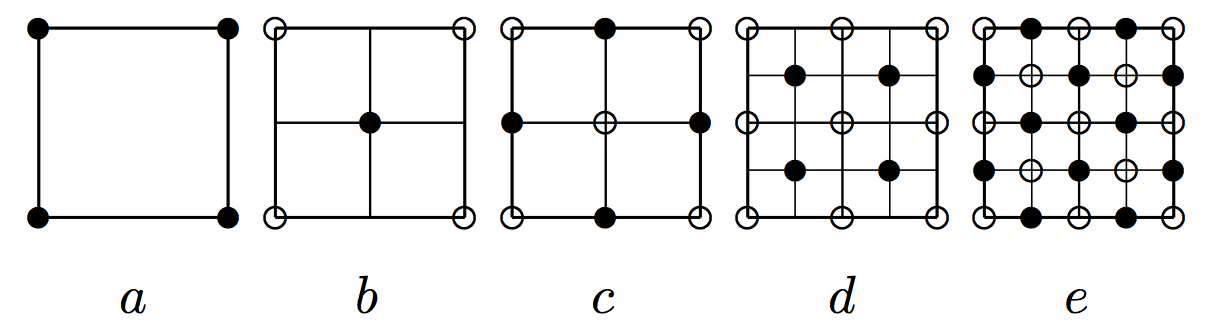
\includegraphics[width=\textwidth]{data/DS.png}
				\vspace{-0.5cm}
				\caption{Этапы работы алгоритма Diamond-Square}\label{fig:DS}
			\end{figure}

			Алгоритм включает в себя следующие этапы (отображены на \hyperref[fig:DS]{Рис. 1}):

			\begin{enumerate}[a)]
				\item \textbf{Инициализация}
					Пусть $n$ и $m$ - заданные ширина и высота требуемой карты высот. Чтобы использовать алгоритм для заданного размера требуется создать карту с шириной и высотой равными:
					\[ n' = 2^{\log_2 (max(n,m) - 1)} + 1 \]
					Для каждого углового элемента полученной карты генерируем случайное значение. Диапазон случайных значений в общем случае может быть любым, но в данной работе возьмем его равным $[0, \frac{n + m}{2}]$. В целом данный диапазон не влияет на производительность алгоритма или на возможность его реализации, он может быть и отрицательным, как, например в случае, когда 0 - это уровень моря.
				\item \textbf{Этап Diamond}
					На этом этапе находится центральная точка рассматриваемого квадрата, как среднее значение от его углов:
					\[ m[s/2][s/2] = \frac{m[0][0] + m[0][s] + m[s][0] + m[s][s]}{4} + rand(-R * s, R * s) \]
					где $m$ - это рассматриваемый квадрат, $s$ - количество узлов на ребре квадрата, $R$ - задаваемый коэффициент.
				\item \textbf{Этап Square}
					Здесь рассматривается ромб с вершинами, вычисленными на этапе Diamond. Подход схожий с этапом Diamond, только теперь высчитываются центральные элементы ребер квадрата по двум углам квадрата и двум центральным точкам, одна из которых - центр рассматриваемого квадрата, а вторая центр соседствующего квадрата. Существует проблема на краях генерируемой карты, ведь в таком случае нет центра соседствующего квадрата. В данной работе было принято следующее решение: при отсутствии соседствующего квадрата брать среднее от 3-ех точек - двух вершин и центра рассматриваемого квадрата.
				\item[d-e)] \textbf{Итерации по рассматриваемым квадратам}
					Итерации проходят по строкам и столбцам с шагом $s$:\\
					В каждой итерации по столбцам происходят этапы Square и Diamond, если итерация упирается в край карты, то происходит переход на следующую строку. При достижении правого нижнего угла матрицы значение $s$ обновляется $s = s / 2$ и итерации по строкам и столбцам происходят заново.\\
					Критерий останова: $s = 2$.
			\end{enumerate}

			После выполнения приведенных выше этапов построенная карта обрезается до размера $n \times m$. Для удобства дальнейшей работы муравьиного алгоритма из построенной карты генерируется нормированная карта.

		\subsection{Муравьиный алгоритм}

			Для построения путей роботов до целей был выбран муравьиный алгоритм \cite{ant}. Алгоритм имеет хорошую практическую применимость в такого рода задачах \cite{ant}\cite{ant1}\cite{ant2}. Существуют и прочие алгоритмы, которые весьма подробно описаны в \cite{path}.

			Основная идея алгоритма заключается в следующем:\\ Запустить на карту некоторую популяцию муравьев, которые должны дойти от начальной точки до конечной, при том каждую вершину пути муравей выбирает основываясь на концентрации феромона на вершине. После того, как все муравьи построили путь - они обновляют концентрацию феромона для каждой вершины, которая была задействована в построении пути. Далее запускается следующая популяция муравьев, которая основывается на уже обновленных значениях концентрации феромона.

			Данный алгоритм имеет низкую производительность при использовании его в чистом виде, однако при применении эвристик можно добиться значительного улучшения производительности.

			Основные этапы реализуемого муравьиного алгоритма:
			\begin{enumerate}
				\item Изначально генерируется матрица размера равного размеру карты, содержащая начальные значения концентрации феромонов $\tau_{ij}$. В общем случае значения матрицы случайны и очень близки к нулю, однако в данной работе применена следующая эвристика: \[
					\tau_{ij} = 1 - (\frac{\rho((i,j), target)}{\max_{i,j}(\rho((i,j), target)} + rand(- R, R))
				\]
				где $\rho$ - это двумерное Евклидово расстояние, $target$ - цель, $0 < R < 1$ - это задаваемое значение шума (вносится для того, чтобы приблизить эвристику к общему подходу). Если полученное значение $< 0$, то $\tau_{ij} = 0$.\\
				\item Популяция муравьев помещается в начальную координату робота.
				\item Следующая вершина карты выбирается случайно. Вероятность выбора вершины $j$ в общем случае задается следующей формулой:
				\[
					p_{ij}^{k}(t) = \frac{\tau_{ij}^{\alpha}(t)}{\sum\limits_{j \in N_{i}^{k}}\tau_{ij}^{\alpha}(t)}
				\]
				Здесь $i$ -- вершина в настоящий момент, $N_{j}^{k}$ -- список доступных вершин, $\alpha$ -- параметр определяющий влияние концентрации феромона на результат, $t$ - текущая итерация алгоритма. \\
				Для достижения лучшей производительности используются две эвристики: \\
				\begin{itemize}
					\item Эвристика по расстоянию\\
						Значение эвристики $\eta_{d\ ij}$ рассчитывается по следующей формуле:
						\begin{gather*}
							\eta_{d\ ij} = exp((target - \max(|j[0] - target[0]|, |j[1] - target[1]|) - \\
							 - \min_{j \in N_{i}}(target - \max(|j[0] - target[0]|, |j[1] - target[1]|)))
						\end{gather*}
						где $target[0]$ - это координата цели по оси X, а $target[0]$ - это координата цели по оси Y. так же и с точкой $j$. В общем случае можно было использовать любое число в основании степенной функции, потому что это требуется исключительно для того чтобы избежать нулевой вероятности.\\
					\item Эвристика по высоте\\
						Значение эвристики $\eta_{d\ ij}$ рассчитывается по следующей формуле:
						\[
							\eta_{h\ ij} = 1 - |m[j[0]][j[1]] - m[i[0]][i[1]]|
						\]
						где m - это сгенерированная карта местности.
				\end{itemize}
				Таким образом вероятность выбора вершины $j$ с учетом эвристик задается формулой:
				\[
					p_{ij}^{k}(t) = \frac{\tau_{ij}^{\alpha}(t)\eta_{d\ ij}^{\beta}\eta_{h\ ij}}{\sum\limits_{j \in N_{i}^{k}}\tau_{ij}^{\alpha}(t)\eta_{d\ ij}^{\beta}\eta_{h\ ij}}
				\]
				\item После прохода всего пути всеми муравьями из каждого пути удаляются петли, а концентрация феромона изменяется согласно следующей формуле:
				\[
					\tau_{ij}^{\alpha}(t+1) = (1 - p)\tau_{ij}^{\alpha}(t) + \sum\limits_{k = 1}^{n_{k}}\frac{q}{L_{k}(t)}
				\]
				Где $p$ определяет скорость испарения феромонов, $n_{k}$ -- это количество муравьев, $L_{k}(t)$ -- длина пройденного муравьем пути, $q$ - задаваемый параметр.
				\item Итерации продолжаются до достижения критерия остановки, который в данном случае задается указанием количества итераций.
			\end{enumerate}

		Данный алгоритм имеет временную сложность $O(t_{n} p_{n} n^{4})$, где $t_{n}$ - количество итераций алгоритма, $p_{n}$ - размер популяции, $n$ - количество узлов на ребре карты высот.

		\subsection{Алгоритм коллективного распределения целей}

		Алгоритм коллективного распределения целей достаточно подробно описан в \cite{plan}. Идея заключается в том, чтобы назначить цель роботу только в том случае, если оценка эффективности для достижения роботом цели выше чем до других целей и выше, чем для других роботов и этой цели.

		Путь имеется $N$ роботов и соответственно такое же число целей.
		Задачу можно записать следующим образом:
		\[
			Y_{c} = \sum_{j = 1}^{N} \sum_{l = 1}^{N} d_{j,l}n_{j,l} \rightarrow max
		\]
		где $n_{j,l}$ определяется при ограничении:
		\[
			\sum_{l=1}^{N} n_{j,l} \leq 1, j = 1, ... , N
		\]
		В качестве оценки эффективности будем использовать Евклидово расстояние от начальной координаты робота до цели.\\
		Алгоритм заключается в следующем:
		\begin{enumerate}
			\item Роботы делают попытку выбора целей в порядке возрастания номеров.
			\item Каждый робот может выбирать не более, чем одну цель, после чего не участвует в выборе целей в данной реализации итерационной процедуры.
			\item Цель, для которой выполняется условие:
				\[
					\sum_{j=1}^{N} n_{j, l} < n_{l}^{max}, \; l \in [1, M], \; n_{l}^{max} = 1, 2, 3, ...
				\]
				т. е. необеспеченная цель, выбирается роботом, еще не выбравшим какую-либо цель, для которого оценка эффективности dj,l этой цели имеет наибольшее значение по сравнению с другими роботами, не выбравшими свои цели.
			\item Если на момент выбора цели j-м роботом группы имеется
			несколько необеспеченных целей, имеющих для данного робота одинаковые значения оценки эффективности, то робот выбирает только одну цель, в соответствии с заранее определeнным правилом, одинаковым для всех роботов данной группы. Например, он может выбирать цель с наименьшим номером. Другими словами, если:
			\begin{gather*}
					d_{j,l_{1}} = d_{j,l_{2}} = ... = d_{j,l_{i}} \\
					l_{1} < l_{2} < ... < l_{i}
			\end{gather*}
			И выполняется условие из предыдущего пункта, то j-м роботом выбирается цель с номером $l_{1}$, т. е. $i_{j}$ = $l{1}$.
			\item Если несколько роботов имеют одинаковые значения оценки эффективности для l-й цели $(l \in [1, M])$ при условии, что она не обеспечена, то выбор этой цели осуществляется роботом с наименьшим номером.
			\item   Если максимальное значение оценки эффективности
			$ d_{k^{*}l^{*}} = \max_{k}d_{kl^{*}}$ некоторой цели $T_{l^{*}}$ принадлежит роботу $R_{j}$, делающему выбор, т. е. $k^{*} = j$, то робот Rj выбирает данную цель, полагая $i_{j} = l^{*}$. В противном случае (когда $k^{*} \neq j$) робот $R_{j}$ отказывается от выбора в данном итерационном цикле.
		\end{enumerate}

	\newpage
	\section{Программная реализация}
		Программ написана на языке Python3.7. Для реализации были использованы следующие библиотеки:
		\begin{itemize}
			\item \textit{math};\\
				Библиотека сожержит математические функции. В реализованной программе используется для таких функций, как exp() и ceil().
			\item \textit{numpy};\\
				Библиотека для работы с многомерными массивами. В программе используется как удобный контейнер для хранения матриц и массивов, а также для различного рода взаимодействия с ними.
			\item \textit{bisect};\\
				Библиотека обеспечивает поддержку списка в отсортированном порядке с помощью алгоритма деления пополам. В программе используется в реализации метода рулетки для случайного выбора с заданными весами.
			\item \textit{time};\\
				Библиотека для работы со временем. Используется в реализации измерений времени работы алгоритмов.
			\item \textit{matplotlib};\\
				Графическая библиотека. Используется для построения графиков.
			\item \textit{progressbar}.\\
				Библиотека для вывода в консоль состояния выполнения программы в процентном соотношении. Используется для мониторинга состояния программы во время выполнения, так как программа запускалась для длительных расчетов данный инструмент показался необходимым.
		\end{itemize}

		В качестве среды разработки использовалась Visual Studio Code. Длительные тесты проводились на виртуальной машине предоставляемой компанией Amazon в качестве одной из услуг AWS (Amazon Web Sevices) - Amazon Elastic Compute Cloud (EC2). Была использована виртуальная машина Amazon Linux AMI (1 vCPUs, 2.5 GHz, Intel Xeon Family).

		Все функции и модули программы содержат комментарии.\\
		Главный модуль программы - \textbf{main.py}. В нем содержатся исключительно функции для тестирования программ и параметры для запуска алгоритмов. Также при реализации программы были подобраны оптимальные параметры для инициализации алгоритмов.

		Для инициализации объекта графа, используются следующие значения параметров:\\

		\begin{tabular}{rl}
			\textbf{Коэффициент гладкости карты:} & 0.3\\
			\multirow{2}{*}{\parbox{7cm}{\textbf{Коэффициент зашумленности начального феромона:}}} & 0.1\\
			&
		\end{tabular}

		Для муравьиного алгоритма используются следующие значения параметров:\\

		\begin{tabular}{rl}
			\textbf{Размер популяции:} & 80\\
			\textbf{Количество итераций:} & 10\\
			\multirow{2}{*}{\parbox{5.5cm}{\textbf{Коэффициент влияния концентрации феромона:}}} & \multirow{2}{*}{1.0}\\
			&\\
			\multirow{2}{*}{\parbox{5.6cm}{\textbf{Коэффициент влияния эвристики по расстоянию:}}} & \multirow{2}{*}{1.0}\\
			&\\
			\multirow{2}{*}{\parbox{4.2cm}{\textbf{Коэффициент испарения феромона:}}} & \multirow{2}{*}{0.9}\\
			&\\
			\multirow{2}{*}{\parbox{6cm}{\textbf{Параметр влияния длины пути на значение феромона:}}} & \multirow{2}{*}{100}\\
			&
		\end{tabular}

		Модуль \textbf{graph.py} содержит класс \textit{Graph}, описывающий карту высот, а также все взаимодействующие с ней элементы, такие как матрицы эвристик, матрица концентраций феромонов, нормированная карта высот и пр. . Параметры, определяющие размер карты высот, гладкость карты и зашумленность начальной концентрации феромонов подаются в конструктор класса. Карта высот генерируется в методе класса \textit{generate()}. Взаимодействие с феромонами и эвристиками также определено в этом классе.

		Модуль \textbf{ant.py} содержит два класса: \textit{Ant} и \textit{EAlg}. Параметры, влияющие на поведение муравьиного алгоритма подаются в конструктор класса \textit{EAlg}. Метод этого класса, принимающий в качестве аргументов объект класса \textit{Graph}, начальные координаты пути и конечные координаты пути, выполняет поиск оптимального пути. В этом методе инициализируется объекты класса \textit{Ant}, который непосредственно строит путь на каждой итерации, обновляет феромоны, и т.д. .

		Модуль \textbf{planning.py} содержит функцию \textit{planning}, которая в качестве аргументов принимает объекты классов \textit{Graph} и \textit{EAlg}, размер наборов роботов (целей), а также объекты инструментального характера для работы библиотеки \textit{progressbar}. В данной функции выполняется алгоритм коллективного распределения целей.

		Все модули взаимодействуют с модулем \textbf{tools.py}. В этом модуле функции инструментального характера необходимые как для функционирования основных алгоритмов (например, поиск соседних точек в графе), так и функции для построения графиков и вывода результатов.

		Полный листинг программы можно посмотреть в \hyperref[sec:code]{ПРИЛОЖЕНИЕ А}.

	\newpage
	\section{Результаты}

	В данном разделе представлены непосредственно результаты работы реализованной программы, а также их исследование.
		\subsection{Diamond-Square}

		Было необходимо сгенерировать карты размером $25 \times 25$,
		$50 \times 50$, $100 \times 100$, $500 \times 500$, $1000 \times 1000$. Результаты работы алгоритма Diamond-Square представлены на \hyperref[fig:map25]{Рис. 2-7}.
			\begin{figure}[H]
				\centering
				\vspace{-0.5cm}
				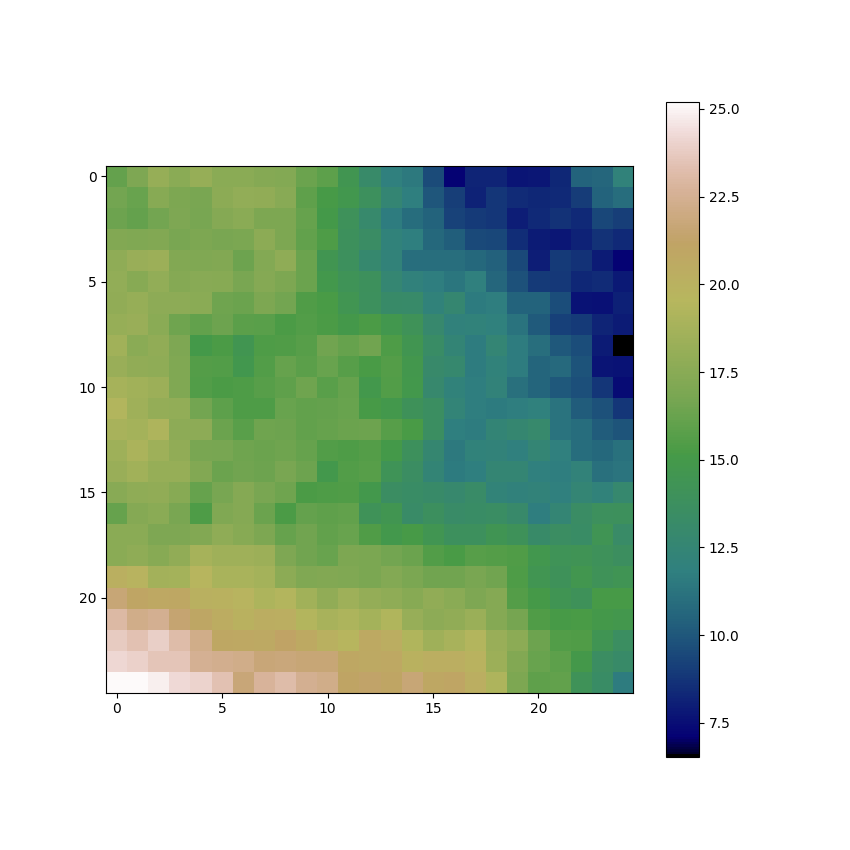
\includegraphics[width=0.6\textwidth]{data/maps_example/25x25.png}
				\vspace{-0.5cm}
				\caption{Карта размера 25x25}\label{fig:map25}
			\end{figure}

			\begin{figure}[H]
				\centering
				\vspace{-0.5cm}
				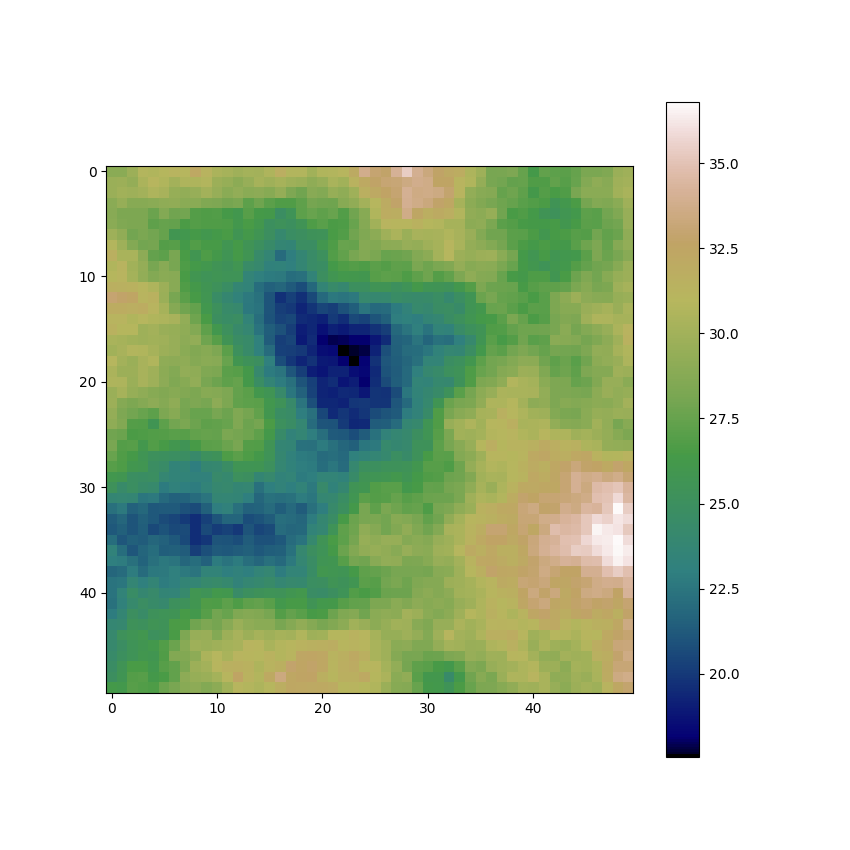
\includegraphics[width=0.6\textwidth]{data/maps_example/50x50.png}
				\vspace{-0.5cm}
				\caption{Карта размера 50x50}\label{fig:map50}
			\end{figure}

			\begin{figure}[H]
				\centering
				\vspace{-0.5cm}
				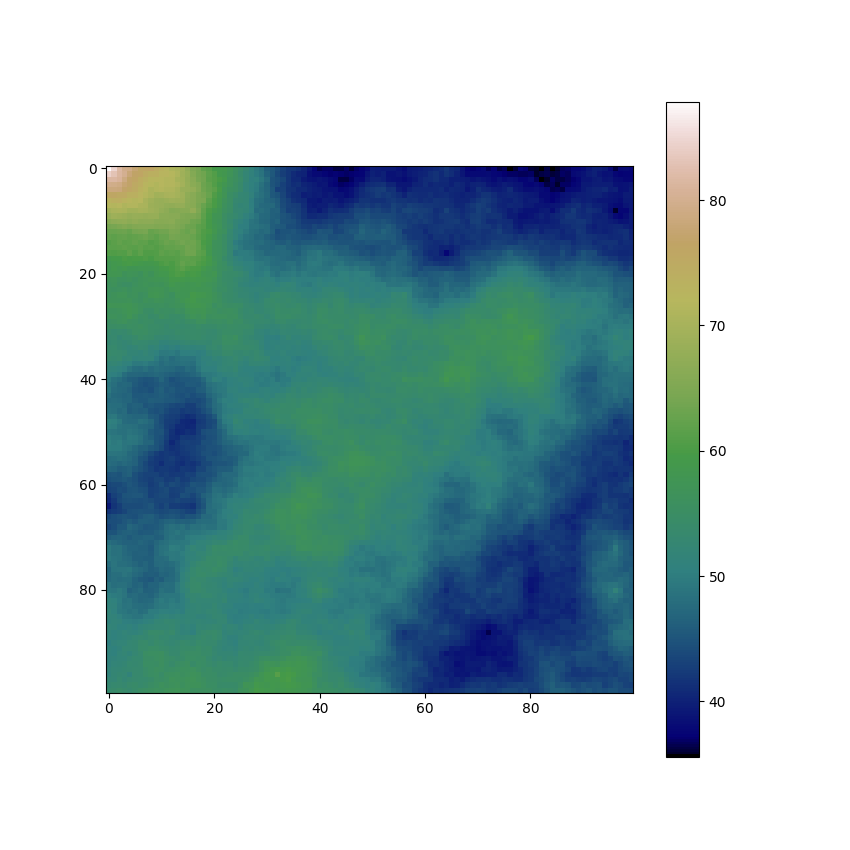
\includegraphics[width=0.6\textwidth]{data/maps_example/100x100.png}
				\vspace{-0.5cm}
				\caption{Карта размера 100x100}\label{fig:map100}
			\end{figure}

			\begin{figure}[H]
				\centering
				\vspace{-0.5cm}
				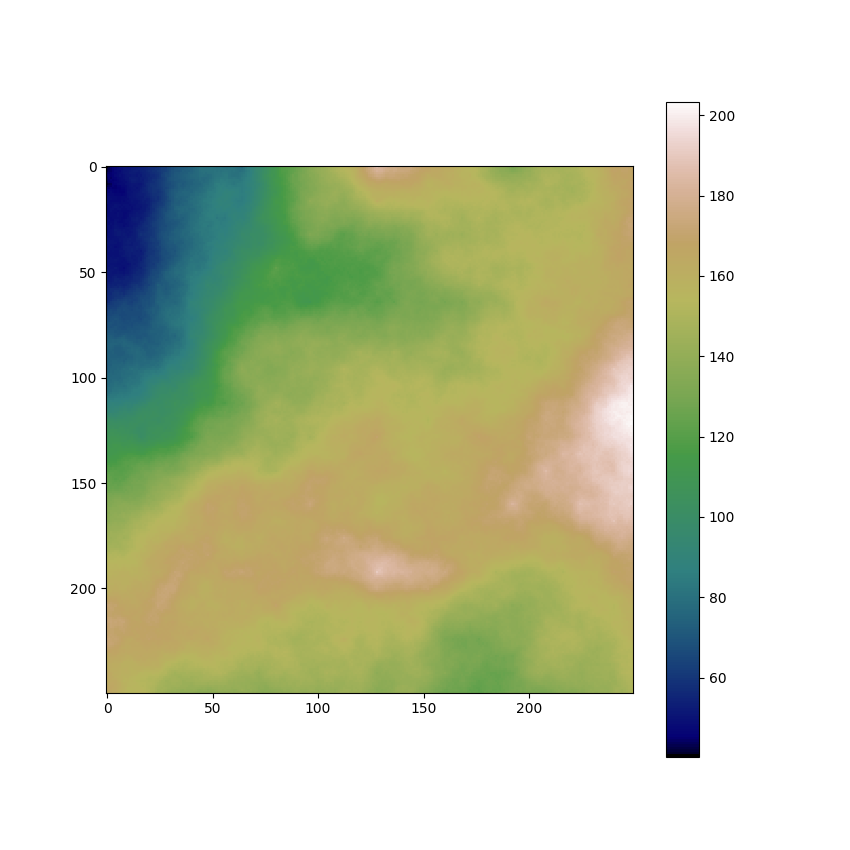
\includegraphics[width=0.6\textwidth]{data/maps_example/250x250.png}
				\vspace{-0.5cm}
				\caption{Карта размера 250x250}\label{fig:map250}
			\end{figure}

			\begin{figure}[H]
				\centering
				\vspace{-0.5cm}
				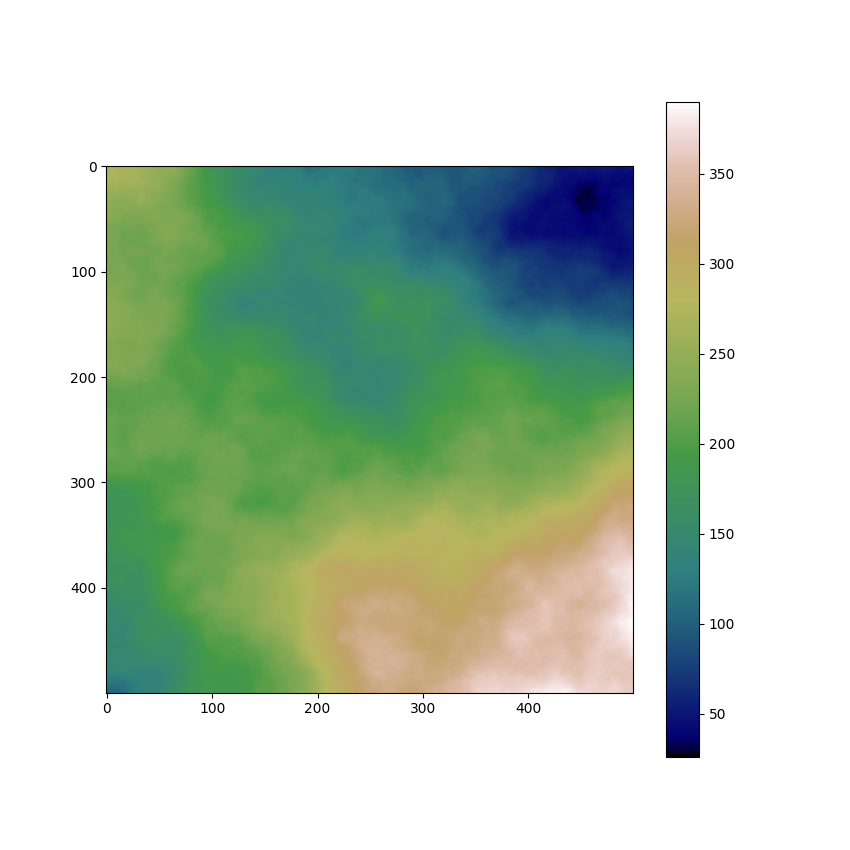
\includegraphics[width=0.6\textwidth]{data/maps_example/500x500.png}
				\vspace{-0.5cm}
				\caption{Карта размера 500x500}\label{fig:map500}
			\end{figure}

			\begin{figure}[H]
				\centering
				\vspace{-0.5cm}
				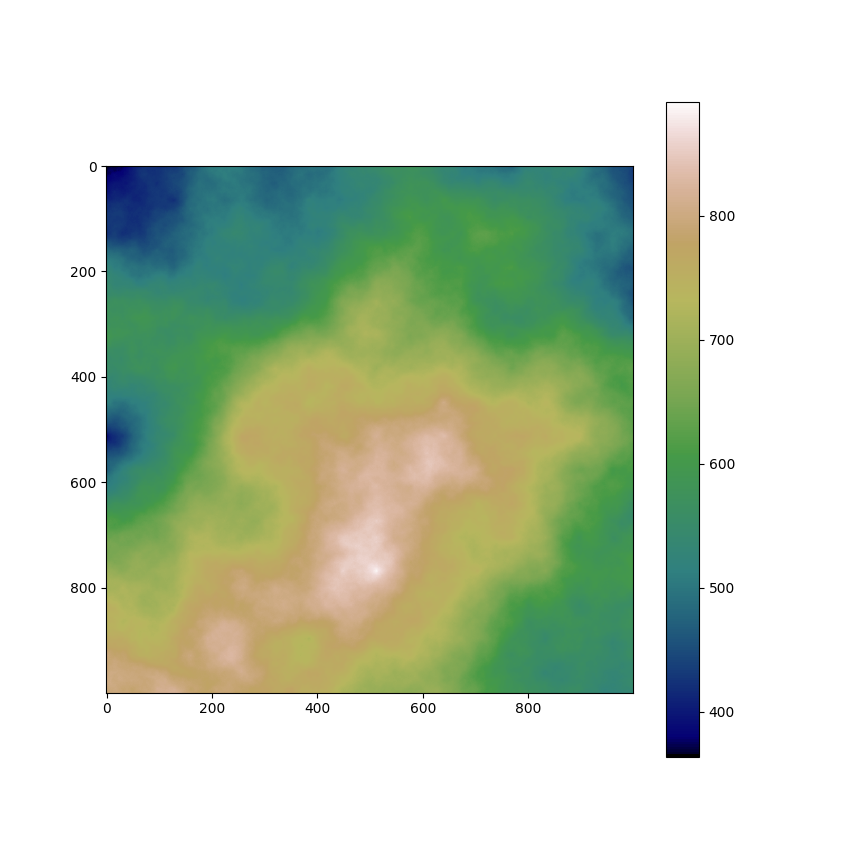
\includegraphics[width=0.6\textwidth]{data/maps_example/1000x1000.png}
				\vspace{-0.5cm}
				\caption{Карта размера 1000x1000}\label{fig:map1000}
			\end{figure}

		\subsection{Муравьиный алгоритм}

			Так как реализованный алгоритм отличается от классического представления муравьиного алгоритма использованием эвристик, то имеет смысл продемонстрировать генерируемые в процессе работы программы карты эвристики. Так как эвристика по высоте определяется только в зависимости от координат соседних точек, то ее сложно представить в виде графика. На \hyperref[fig:heur_d]{Рис. 8} представлены карты эвристики по расстоянию для разного размера карты высот и разных целевых точек.

			\begin{figure}[H]
				\vspace{-0.5cm}
				\centering
				\begin{subfigure}[b]{0.49\textwidth}
					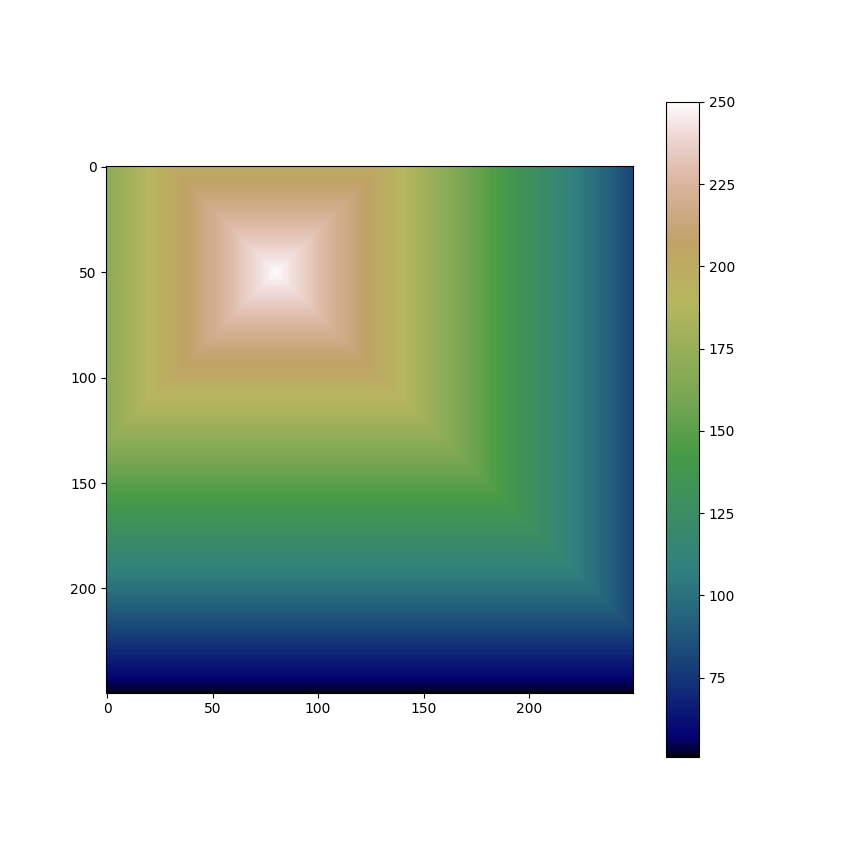
\includegraphics[width=\textwidth]{data/heuristics_example/heuristic_d_250x250.png}
					\caption*{Карта 250x250, Цель ([180, 200)}
				\end{subfigure}
				\begin{subfigure}[b]{0.49\textwidth}
					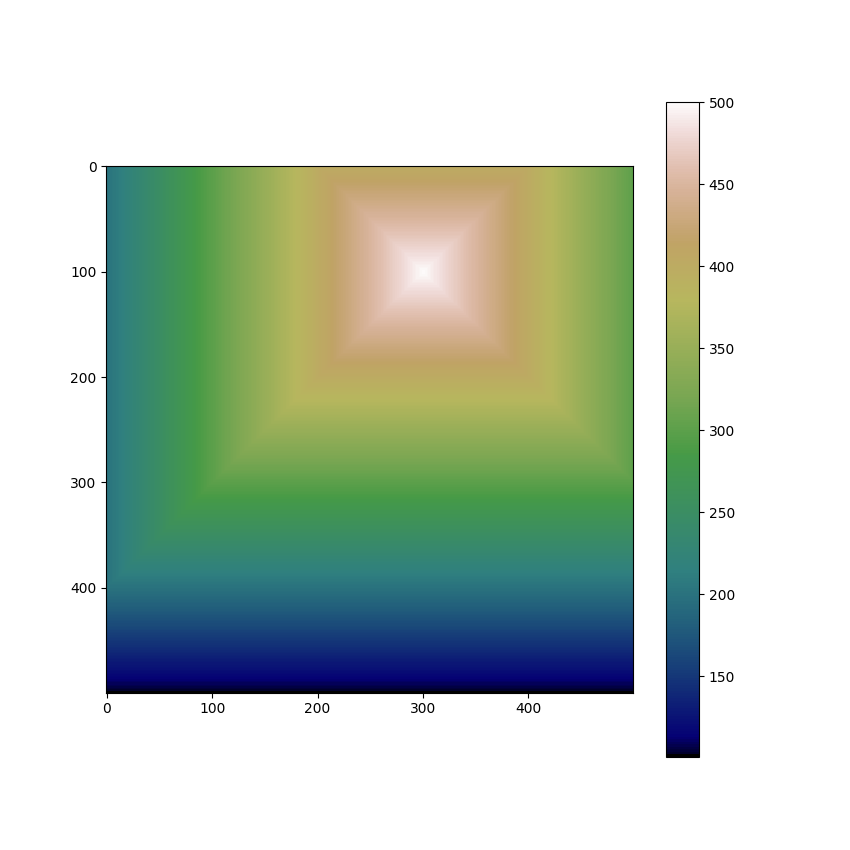
\includegraphics[width=\textwidth]{data/heuristics_example/heuristic_d_500x500.png}
					\caption*{Карта 500x500, Цель (100, 300)}
				\end{subfigure}
				\caption{Эвристики по расстоянию}\label{fig:heur_d}
			\end{figure}

			На \hyperref[fig:pher]{Рис. 9} представлены карты начальной концентрации феромонов для разного размера карты высот и разных целевых точек. Карты зашумлены для приближения работы алгоритма в начальной итерации к общему случаю с случайными значениями концентрации феромонов.

			\begin{figure}[H]
				\vspace{-0.5cm}
				\centering
				\begin{subfigure}[b]{0.49\textwidth}
					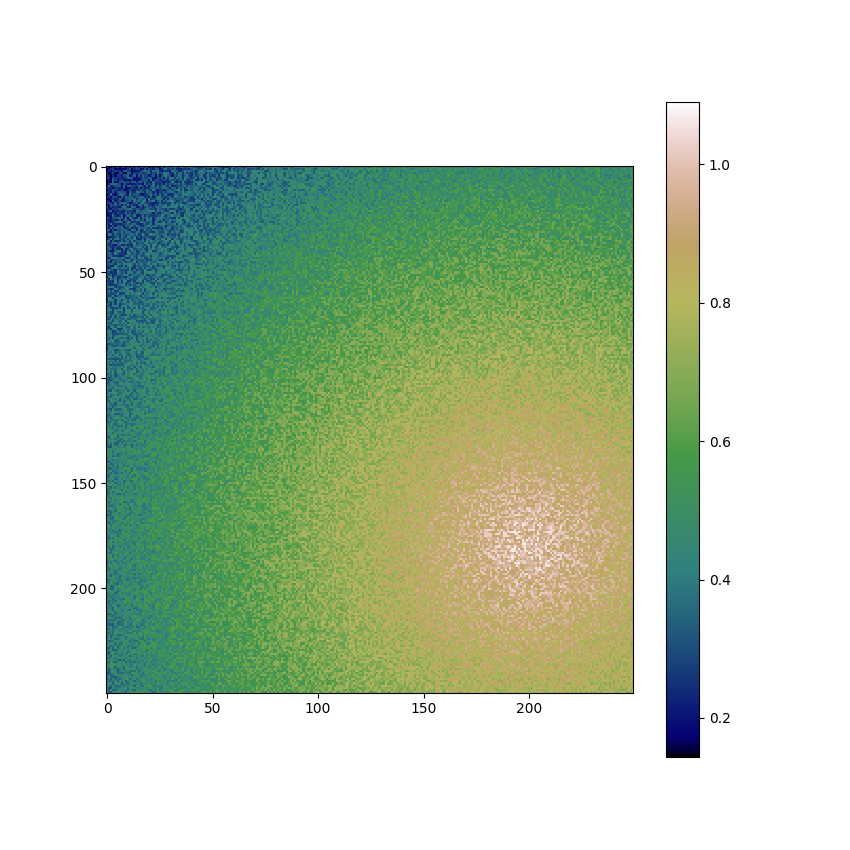
\includegraphics[width=\textwidth]{data/heuristics_example/pheromone_250x250.png}
					\caption*{Карта 250x250, Цель (50, 80)}
				\end{subfigure}
				\begin{subfigure}[b]{0.49\textwidth}
					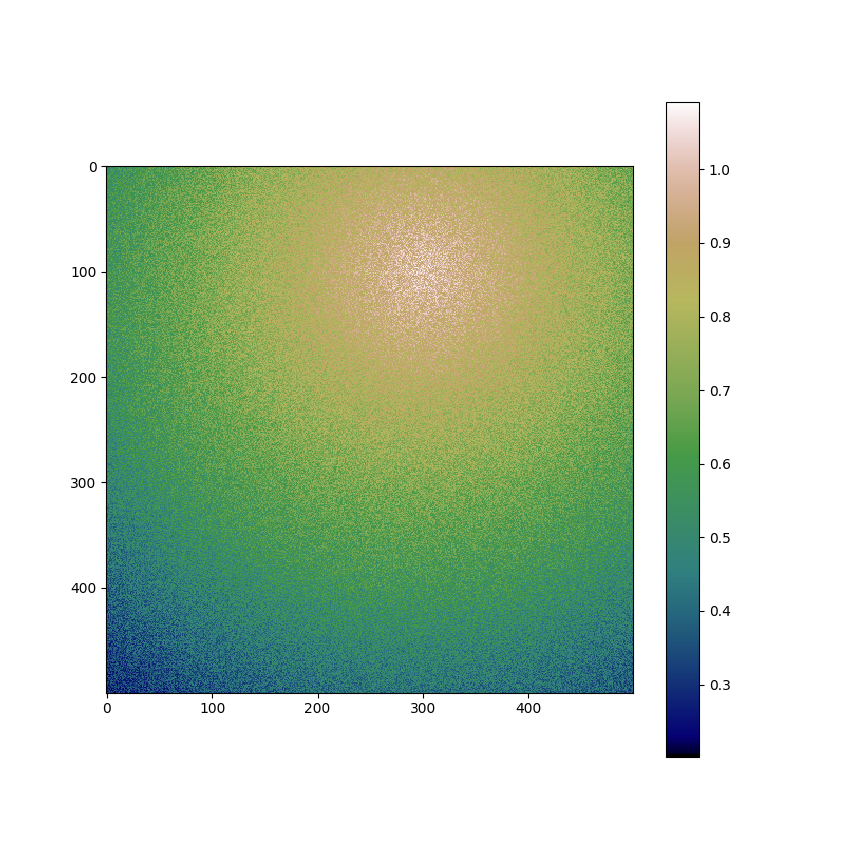
\includegraphics[width=\textwidth]{data/heuristics_example/pheromone_500x500.png}
					\caption*{Карта 500x500, Цель (345, 345)}
				\end{subfigure}
				\caption{Начальная концентрация феромонов}\label{fig:pher}
			\end{figure}

			На \hyperref[fig:rob1]{Рис. 10-11} представлены результаты поиска пути для этих эвристик и начальных феромонов. Начальная координата - черная, конечная - красная.

			\begin{figure}[H]
				\centering
				\vspace{-0.5cm}
				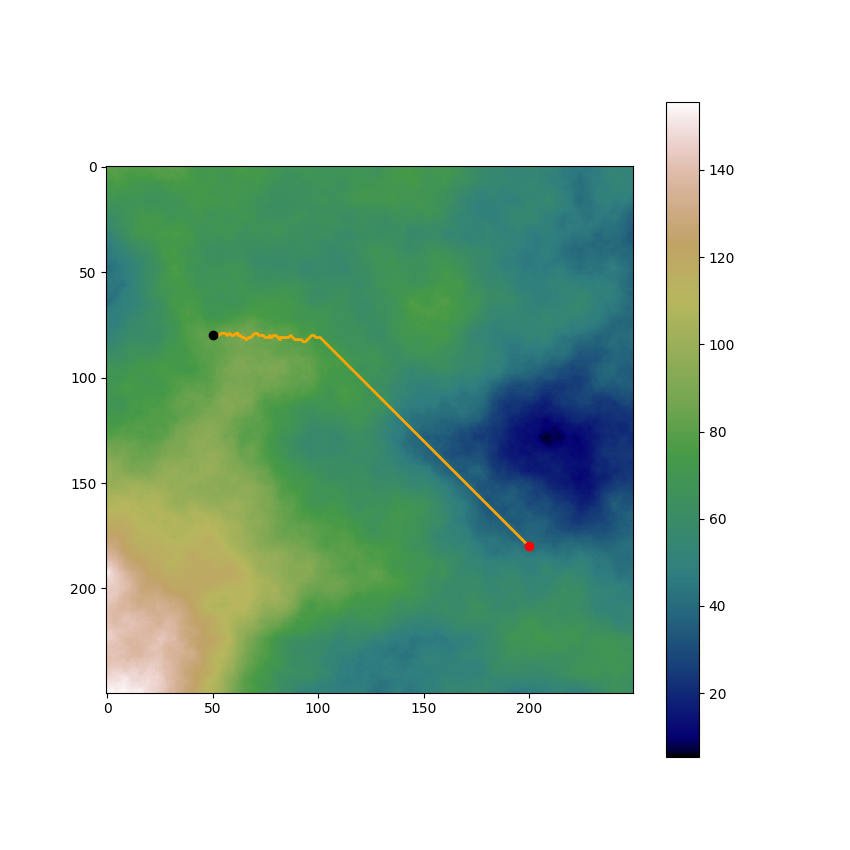
\includegraphics[width=0.6\textwidth]{data/path_example/250x250.png}
				\vspace{-0.5cm}
				\caption{Построенный путь для робота на карте размера 250x250}\label{fig:rob1}
			\end{figure}

			\begin{figure}[H]
				\centering
				\vspace{-0.5cm}
				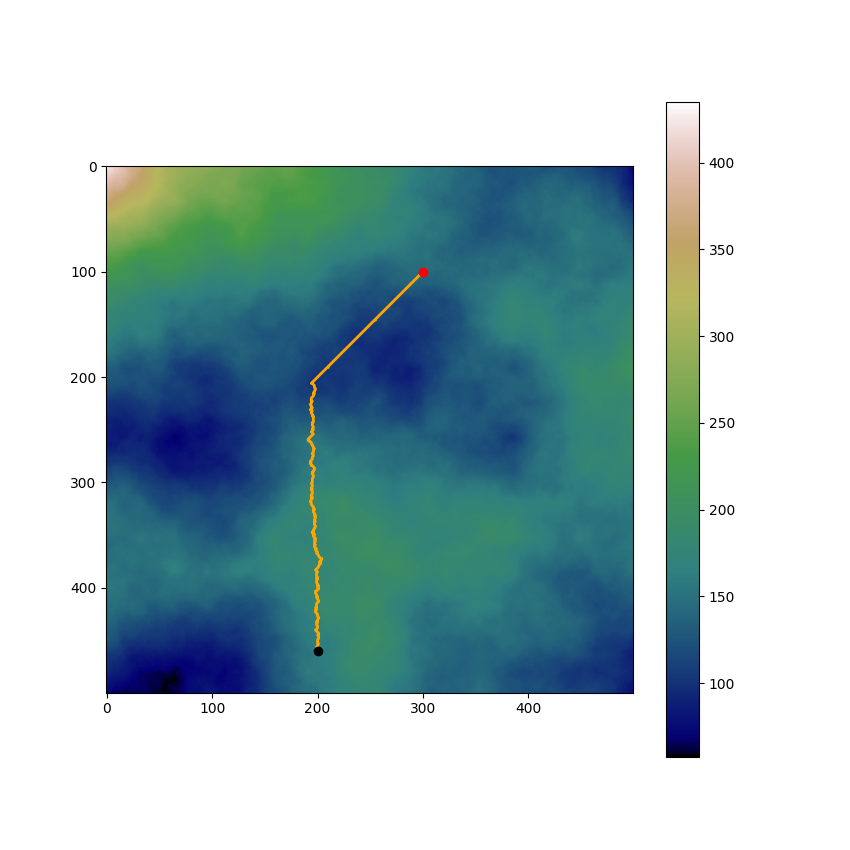
\includegraphics[width=0.6\textwidth]{data/path_example/500x500.png}
				\vspace{-0.5cm}
				\caption{Построенный путь для робота на карте размера 500x500}\label{fig:rob2}
			\end{figure}

		\subsection{Коллективное распределение целей}

			Примеры результатов работы алгоритма коллективного распределения целей представлены на \hyperref[fig:5robs]{Рис. 12-13}.

			\begin{figure}[H]
				\centering
				\vspace{-0.5cm}
				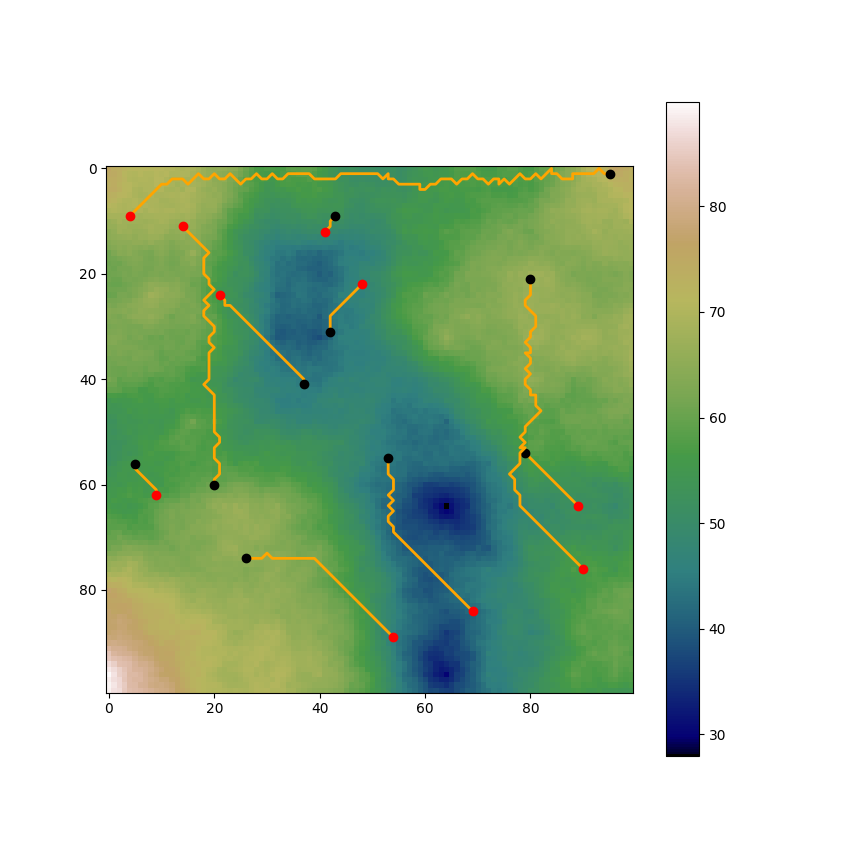
\includegraphics[width=0.6\textwidth]{data/mean_paths/100x100/10.png}
				\vspace{-0.5cm}
				\caption{Построенные пути для 10 роботов на карте размера 100x100}\label{fig:5robs}
			\end{figure}

			\begin{figure}[H]
				\centering
				\vspace{-0.5cm}
				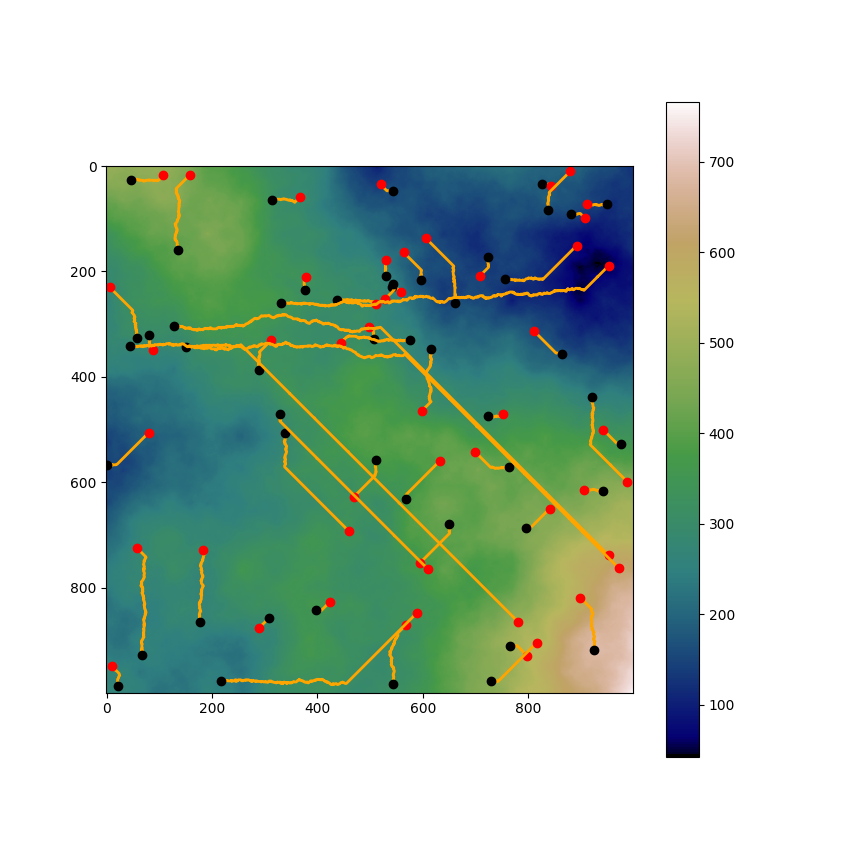
\includegraphics[width=0.6\textwidth]{data/mean_paths/1000x1000/50.png}
				\vspace{-0.5cm}
				\caption{Построенные пути для 50 роботов на карте размера 1000x1000}\label{fig:50robs}
			\end{figure}

		\subsection{Исследования временной сложности алгоритмов}

			На \hyperref[fig:time_surface]{Рис. 14} представлена плоскость отображающая зависимость времени вычислений от количества роботов и размера карты. На плоскости отображены только средние элементы измерений времени, полную информацию о измерении времени можно найти в \hyperref[sec:time]{ПРИЛОЖЕНИЕ Б}. Для наглядности ось по времени представлена в виде логарифмической шкалы.

			\begin{figure}[H]
				\centering
				\vspace{-0.5cm}
				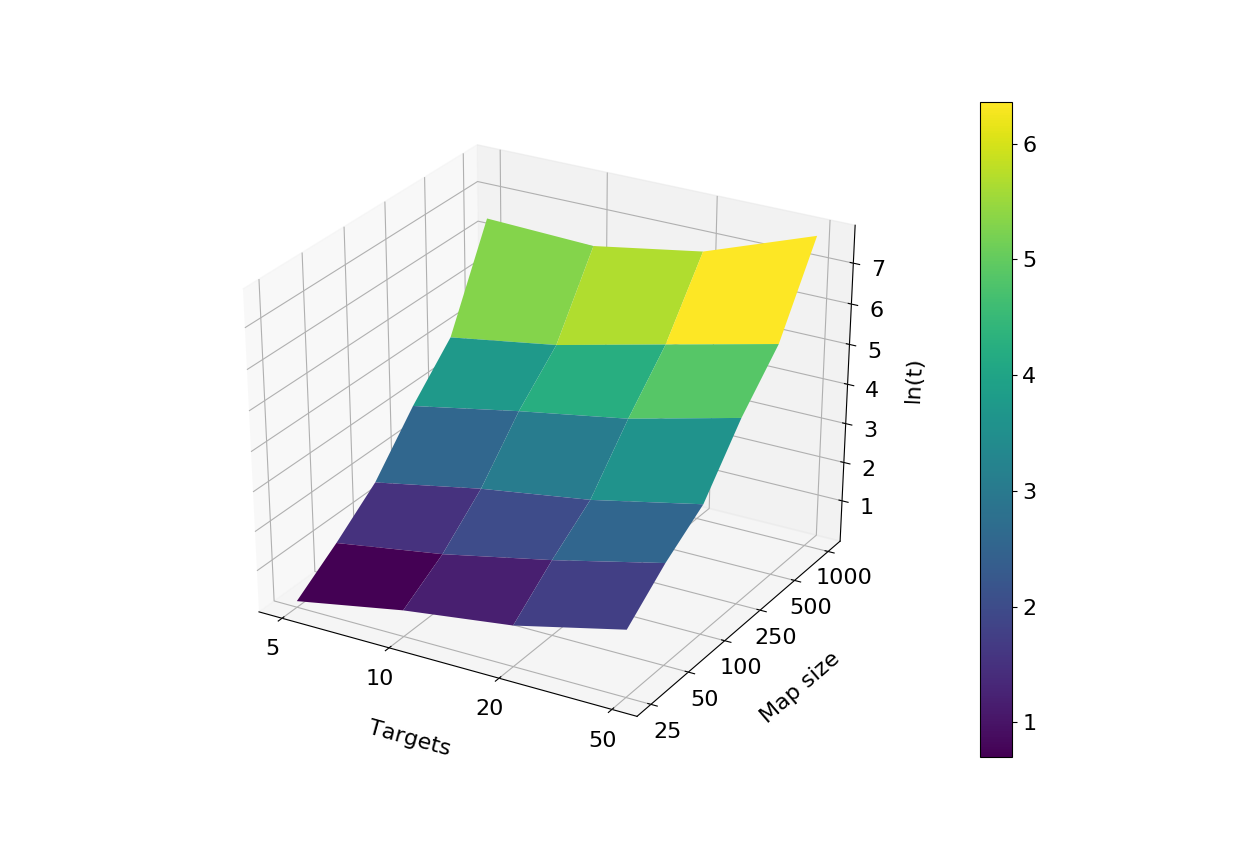
\includegraphics[width=\textwidth]{data/mean_surface.png}
				\vspace{-0.5cm}
				\caption{Зависимость времени вычислений (с.) от размера карты и количества роботов}\label{fig:time_surface}
			\end{figure}

			На \hyperref[fig:time_surface]{Рис. 15} представлен график зависимости времени работы муравьиного алгоритма от размера карты при построении одного пути. Как можно заметить, временная сложность приблизительно квадратичная. Снижение сложности по сравнению с теоретической сложностью алгоритма аргументируется использованием эвристик и оптимального подбора параметров.

			\begin{figure}[H]
				\centering
				\vspace{-0.5cm}
				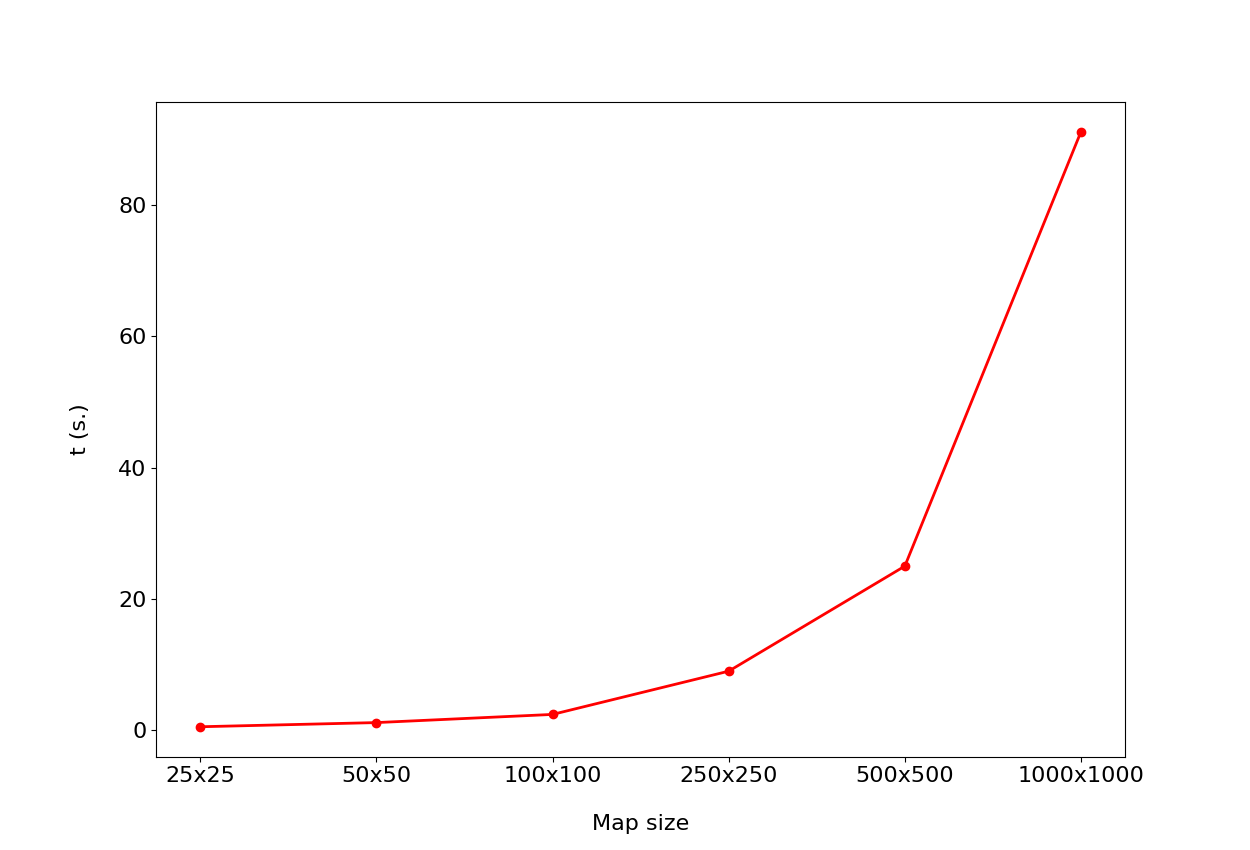
\includegraphics[width=\textwidth]{data/path_time.png}
				\vspace{-0.5cm}
				\caption{Зависимость времени вычислений одного пути (с.) от размера карты}\label{fig:time_path}
			\end{figure}

			Практические результаты действительно отображают, что наибольшее влияние на время выполнение оказывает размер карты высот и меньшее влияние, однако все равно ощутимое, оказывает количество роботов. Общее время вычислений составило $\approx$ 14 часов. Так как время выполнения теста уже с таким количеством вариаций внушительное, то генерация 10-ти разных наборов данных для каждой карты и каждого количества роботов была опущена.

			Из таблиц в \hyperref[sec:time]{ПРИЛОЖЕНИЕ Б} также можно сделать вывод о том, что влияние оказываемое алгоритмом распределения целей на общую работу программы минимально и время его работы зависит от количества роботов.

    \newpage
    \addcontentsline{toc}{section}{ЗАКЛЮЧЕНИЕ}
	\section*{ЗАКЛЮЧЕНИЕ}

	В рамках выполнения курсовой работы были выполнены следующие задачи:
	\begin{itemize}
		\item Генерация карт размеров 25x25, 50x50, 100x100, 250x250, 500x500, 1000x1000 с помощью алгоритма Diamond-Square;
		\item Были распределены цели по роботам используя алгоритм коллективного распределения целей для численностей 5, 10, 20 и 50;
		\item Для роботов были построены оптимальные пути используя муравьиный алгоритм.
	\end{itemize}

	В работе проведено исследование сложностей алгоритмов. Теоретическая сложность муравьиного алгоритма $O(t_{n} p_{n} n^{4})$. Однако результат значительно улучшается с помощью эвристик. Эвристики необходимы для решения проблемы низкой сходимости муравьиного алгоритма. Также в ходе работы были подобраны оптимальные параметры для работы муравьиного алгоритма.

	При измерении времени работы программы была выявлена линейная зависимость времени выполнения от размера карты высот. Учитывая предыдущий вывод о сложности муравьиного алгоритма можно сделать вывод, что алгоритм коллективного распределения целей значительно сэкономил время работы программы. Сложность
	этого алгоритма является пропорциональной количеству роботов (целей).

	Таким образом, учитывая, что рассмотренный алгоритм распределения целей весьма низкозатратен (время выполнения менее доли секунды), но при этом значительно улучшает суммарное время работы программы, то его практическая применимость в подобного рода задачах не стоит под вопросом.

    \newpage
	\renewcommand\refname{ЛИТЕРАТУРА}
	\addcontentsline{toc}{section}{ЛИТЕРАТУРА}
	\begin{thebibliography}{}
		\bibitem{terrain} Miguel Monteiro de Sousa Frade. Genetic Terrain Programming // Universidad de Extremadura, 2008, pp. 103
		\bibitem{plan} Каляев И.А. Модели и алгоритмы коллективного управления в группах роботов // Физматлит, 2009, 279с.
		\bibitem{path} Gregor Klančar. Path Planning // Wheeled Mobile Robotics, 2017, pp. 161-206
		\bibitem{DS} Jacob Olsen. Realtime Procedural Terrain Generation // University of Southern Denmark, 2004, pp. 20
		\bibitem{ant} M. Brand, M. Masuda, N. Wehner, X.-H. Yu. Ant colony optimization algorithm for robot path planning // Computer Design and Applications (ICCDA) 2010 International Conference on, vol. 3, 2010, pp. 436-440.
		\bibitem{ant1} Alpa Reshamwala, Deepika P Vinchurkar. Robot Path Planning using An Ant Colony Optimization Approach: A Survey // (IJARAI) International Journal of Advanced Research in Artificial Intelligence, Vol. 2, No.3, 2013, pp. 7
		\bibitem{ant2} Sangita Sarangi. Optimization of Robot Motion Planning using Ant Colony Optimization // National Institute of Technology, Rourkela, 2011, pp. 81
	\end{thebibliography}


    \newpage
    \addcontentsline{toc}{section}{ПРИЛОЖЕНИЕ А. Исходный код}
	\section*{ПРИЛОЖЕНИЕ А. Исходный код} \label{sec:code}
	Ниже приведен исходный код на языке Python
	\lstinputlisting[language = python, style=style, title={main.py}]{data/code/main.py}
	\lstinputlisting[language = python, style=style, title={graph.py}]{data/code/graph.py}
	\lstinputlisting[language = python, style=style, title={ant.py}]{data/code/ant.py}
	\lstinputlisting[language = python, style=style, title={planning.py}]{data/code/planning.py}
	\lstinputlisting[language = python, style=style, title={tools.py}]{data/code/tools.py}


    \newpage
    \addcontentsline{toc}{section}{ПРИЛОЖЕНИЕ Б. Таблицы измерений времени}
	\section*{ПРИЛОЖЕНИЕ Б. Таблицы измерений времени} \label{sec:time}
	Ниже приведены измерения времени (c.) муравьиного алгоритма для каждой сгенерированной карты и каждого количества роботов:

	\begin{table}[H]
\centering
\begin{tabular}{|r|l|l|l|l|}
\hline
№ карты\textbackslash Кол-во роботов & \textbf{5} & \textbf{10} & \textbf{20} & \textbf{50}\\ \hline
1 & 0.0 & 0.0 & 0.0 & 0.004\\ \hline
2 & 0.0 & 0.0 & 0.001 & 0.004\\ \hline
3 & 0.0 & 0.0 & 0.0 & 0.005\\ \hline
4 & 0.0 & 0.0 & 0.001 & 0.003\\ \hline
5 & 0.0 & 0.0 & 0.0 & 0.004\\ \hline
6 & 0.0 & 0.0 & 0.0 & 0.004\\ \hline
7 & 0.0 & 0.0 & 0.0 & 0.004\\ \hline
8 & 0.0 & 0.0 & 0.0 & 0.004\\ \hline
9 & 0.0 & 0.0 & 0.0 & 0.004\\ \hline
10 & 0.0 & 0.0 & 0.0 & 0.005\\ \hline
Средний элемент & 0.0 & 0.0 & 0.0 & 0.004\\ \hline
\end{tabular}
\caption*{Размер карты: 25x25}
\end{table}

	\begin{table}[H]
\centering
\begin{tabular}{|r|l|l|l|l|}
\hline
№ карты\textbackslash Кол-во роботов & \textbf{5} & \textbf{10} & \textbf{20} & \textbf{50}\\ \hline
1 & 0.0 & 0.0 & 0.001 & 0.005\\ \hline
2 & 0.0 & 0.0 & 0.0 & 0.003\\ \hline
3 & 0.0 & 0.0 & 0.0 & 0.004\\ \hline
4 & 0.0 & 0.0 & 0.0 & 0.004\\ \hline
5 & 0.0 & 0.0 & 0.001 & 0.003\\ \hline
6 & 0.0 & 0.0 & 0.001 & 0.004\\ \hline
7 & 0.0 & 0.0 & 0.0 & 0.004\\ \hline
8 & 0.0 & 0.0 & 0.0 & 0.003\\ \hline
9 & 0.0 & 0.0 & 0.0 & 0.004\\ \hline
10 & 0.0 & 0.0 & 0.0 & 0.004\\ \hline
Средний элемент & 0.0 & 0.0 & 0.0 & 0.004\\ \hline
\end{tabular}
\caption*{Размер карты: 50x50}
\end{table}

	\begin{table}[H]
\centering
\begin{tabular}{|r|l|l|l|l|}
\hline
№ карты\textbackslash Кол-во роботов & \textbf{5} & \textbf{10} & \textbf{20} & \textbf{50}\\ \hline
1 & 6.32895 & 8.73452 & 14.94095 & 24.71504\\ \hline
2 & 5.26532 & 9.12678 & 13.68367 & 30.10719\\ \hline
3 & 4.87571 & 12.12137 & 14.66411 & 26.09427\\ \hline
4 & 5.98595 & 7.40209 & 12.80597 & 23.22383\\ \hline
5 & 3.94488 & 10.1101 & 17.56255 & 28.4082\\ \hline
6 & 7.12389 & 8.61739 & 13.43984 & 25.22285\\ \hline
7 & 5.36162 & 8.51896 & 13.89583 & 25.27979\\ \hline
8 & 5.02578 & 9.56457 & 11.74729 & 23.15173\\ \hline
9 & 5.34449 & 13.91983 & 14.71402 & 22.08825\\ \hline
10 & 6.81967 & 9.45882 & 17.0239 & 31.06226\\ \hline
Средний элемент & 5.34449 & 9.12678 & 13.89583 & 25.22285\\ \hline
\end{tabular}
\caption*{Размер карты: 100x100}
\end{table}

	\begin{table}[H]
\centering
\begin{tabular}{|r|l|l|l|l|}
\hline
№ карты\textbackslash Кол-во роботов & \textbf{5} & \textbf{10} & \textbf{20} & \textbf{50}\\ \hline
1 & 42.28 & 32.36 & 52.149 & 107.196\\ \hline
2 & 19.016 & 27.002 & 69.753 & 103.928\\ \hline
3 & 20.361 & 30.919 & 45.16 & 103.125\\ \hline
4 & 17.649 & 38.522 & 52.348 & 115.323\\ \hline
5 & 19.154 & 39.692 & 60.4 & 123.056\\ \hline
6 & 25.561 & 25.462 & 49.701 & 121.093\\ \hline
7 & 18.231 & 34.012 & 58.345 & 93.992\\ \hline
8 & 13.386 & 34.576 & 51.704 & 105.007\\ \hline
9 & 17.922 & 35.839 & 48.99 & 98.7\\ \hline
10 & 23.871 & 26.686 & 54.966 & 103.896\\ \hline
Средний элемент & 19.016 & 32.36 & 52.149 & 103.928\\ \hline
\end{tabular}
\caption*{Размер карты: 250x250}
\end{table}

	\begin{table}[H]
\centering
\begin{tabular}{|r|l|l|l|l|}
\hline
№ карты\textbackslash Кол-во роботов & \textbf{5} & \textbf{10} & \textbf{20} & \textbf{50}\\ \hline
1 & 47.88517 & 73.60561 & 137.27325 & 308.64456\\ \hline
2 & 48.11748 & 105.09704 & 167.23236 & 321.9515\\ \hline
3 & 64.0862 & 109.30441 & 143.13767 & 335.52867\\ \hline
4 & 59.32068 & 187.01288 & 168.12613 & 364.50322\\ \hline
5 & 75.32691 & 124.74065 & 178.59087 & 319.94925\\ \hline
6 & 61.19254 & 79.99268 & 128.15281 & 503.20078\\ \hline
7 & 51.79195 & 87.23905 & 198.67009 & 341.6798\\ \hline
8 & 58.80499 & 87.76271 & 282.89796 & 311.80583\\ \hline
9 & 56.37451 & 80.41181 & 277.18092 & 283.16109\\ \hline
10 & 56.46719 & 103.25168 & 243.64185 & 409.125\\ \hline
Средний элемент & 56.46719 & 87.76271 & 168.12613 & 321.9515\\ \hline
\end{tabular}
\caption*{Размер карты: 500x500}
\end{table}

	\begin{table}[H]
\centering
\begin{tabular}{|r|l|l|l|l|}
\hline
№ карты\textbackslash Кол-во роботов & \textbf{5} & \textbf{10} & \textbf{20} & \textbf{50}\\ \hline
1 & 985.467 & 292.7 & 847.499 & 2510.479\\ \hline
2 & 289.546 & 551.286 & 879.198 & 1478.341\\ \hline
3 & 775.556 & 516.55 & 493.118 & 2206.797\\ \hline
4 & 612.462 & 1196.722 & 596.369 & 2167.358\\ \hline
5 & 356.076 & 626.026 & 757.651 & 2049.006\\ \hline
6 & 258.133 & 1190.344 & 1356.154 & 2417.786\\ \hline
7 & 1100.106 & 554.877 & 1412.945 & 2335.377\\ \hline
8 & 715.701 & 372.302 & 1571.88 & 4075.243\\ \hline
9 & 905.145 & 777.733 & 2050.21 & 4158.513\\ \hline
10 & 170.516 & 1581.04 & 2182.638 & 4512.163\\ \hline
Средний элемент & 612.462 & 554.877 & 879.198 & 2335.377\\ \hline
\end{tabular}
\caption*{Размер карты: 1000x1000}
\end{table}


	Ниже приведены измерениыя времени (c.) алгоритма планирования для каждой сгенерированной карты и каждого количества роботов:

	\begin{table}[H]
\centering
\begin{tabular}{|r|l|l|l|l|}
\hline
№ карты\textbackslash Кол-во роботов & \textbf{5} & \textbf{10} & \textbf{20} & \textbf{50}\\ \hline
1 & 0.0 & 0.0 & 0.0 & 0.004\\ \hline
2 & 0.0 & 0.0 & 0.001 & 0.004\\ \hline
3 & 0.0 & 0.0 & 0.0 & 0.005\\ \hline
4 & 0.0 & 0.0 & 0.001 & 0.003\\ \hline
5 & 0.0 & 0.0 & 0.0 & 0.004\\ \hline
6 & 0.0 & 0.0 & 0.0 & 0.004\\ \hline
7 & 0.0 & 0.0 & 0.0 & 0.004\\ \hline
8 & 0.0 & 0.0 & 0.0 & 0.004\\ \hline
9 & 0.0 & 0.0 & 0.0 & 0.004\\ \hline
10 & 0.0 & 0.0 & 0.0 & 0.005\\ \hline
Средний элемент & 0.0 & 0.0 & 0.0 & 0.004\\ \hline
\end{tabular}
\caption*{Размер карты: 25x25}
\end{table}

	\begin{table}[H]
\centering
\begin{tabular}{|r|l|l|l|l|}
\hline
№ карты\textbackslash Кол-во роботов & \textbf{5} & \textbf{10} & \textbf{20} & \textbf{50}\\ \hline
1 & 0.0 & 0.0 & 0.001 & 0.005\\ \hline
2 & 0.0 & 0.0 & 0.0 & 0.003\\ \hline
3 & 0.0 & 0.0 & 0.0 & 0.004\\ \hline
4 & 0.0 & 0.0 & 0.0 & 0.004\\ \hline
5 & 0.0 & 0.0 & 0.001 & 0.003\\ \hline
6 & 0.0 & 0.0 & 0.001 & 0.004\\ \hline
7 & 0.0 & 0.0 & 0.0 & 0.004\\ \hline
8 & 0.0 & 0.0 & 0.0 & 0.003\\ \hline
9 & 0.0 & 0.0 & 0.0 & 0.004\\ \hline
10 & 0.0 & 0.0 & 0.0 & 0.004\\ \hline
Средний элемент & 0.0 & 0.0 & 0.0 & 0.004\\ \hline
\end{tabular}
\caption*{Размер карты: 50x50}
\end{table}

	\begin{table}[H]
\centering
\begin{tabular}{|r|l|l|l|l|}
\hline
№ карты\textbackslash Кол-во роботов & \textbf{5} & \textbf{10} & \textbf{20} & \textbf{50}\\ \hline
1 & 6.32895 & 8.73452 & 14.94095 & 24.71504\\ \hline
2 & 5.26532 & 9.12678 & 13.68367 & 30.10719\\ \hline
3 & 4.87571 & 12.12137 & 14.66411 & 26.09427\\ \hline
4 & 5.98595 & 7.40209 & 12.80597 & 23.22383\\ \hline
5 & 3.94488 & 10.1101 & 17.56255 & 28.4082\\ \hline
6 & 7.12389 & 8.61739 & 13.43984 & 25.22285\\ \hline
7 & 5.36162 & 8.51896 & 13.89583 & 25.27979\\ \hline
8 & 5.02578 & 9.56457 & 11.74729 & 23.15173\\ \hline
9 & 5.34449 & 13.91983 & 14.71402 & 22.08825\\ \hline
10 & 6.81967 & 9.45882 & 17.0239 & 31.06226\\ \hline
Средний элемент & 5.34449 & 9.12678 & 13.89583 & 25.22285\\ \hline
\end{tabular}
\caption*{Размер карты: 100x100}
\end{table}

	\begin{table}[H]
\centering
\begin{tabular}{|r|l|l|l|l|}
\hline
№ карты\textbackslash Кол-во роботов & \textbf{5} & \textbf{10} & \textbf{20} & \textbf{50}\\ \hline
1 & 42.28 & 32.36 & 52.149 & 107.196\\ \hline
2 & 19.016 & 27.002 & 69.753 & 103.928\\ \hline
3 & 20.361 & 30.919 & 45.16 & 103.125\\ \hline
4 & 17.649 & 38.522 & 52.348 & 115.323\\ \hline
5 & 19.154 & 39.692 & 60.4 & 123.056\\ \hline
6 & 25.561 & 25.462 & 49.701 & 121.093\\ \hline
7 & 18.231 & 34.012 & 58.345 & 93.992\\ \hline
8 & 13.386 & 34.576 & 51.704 & 105.007\\ \hline
9 & 17.922 & 35.839 & 48.99 & 98.7\\ \hline
10 & 23.871 & 26.686 & 54.966 & 103.896\\ \hline
Средний элемент & 19.016 & 32.36 & 52.149 & 103.928\\ \hline
\end{tabular}
\caption*{Размер карты: 250x250}
\end{table}

	\begin{table}[H]
\centering
\begin{tabular}{|r|l|l|l|l|}
\hline
№ карты\textbackslash Кол-во роботов & \textbf{5} & \textbf{10} & \textbf{20} & \textbf{50}\\ \hline
1 & 47.88517 & 73.60561 & 137.27325 & 308.64456\\ \hline
2 & 48.11748 & 105.09704 & 167.23236 & 321.9515\\ \hline
3 & 64.0862 & 109.30441 & 143.13767 & 335.52867\\ \hline
4 & 59.32068 & 187.01288 & 168.12613 & 364.50322\\ \hline
5 & 75.32691 & 124.74065 & 178.59087 & 319.94925\\ \hline
6 & 61.19254 & 79.99268 & 128.15281 & 503.20078\\ \hline
7 & 51.79195 & 87.23905 & 198.67009 & 341.6798\\ \hline
8 & 58.80499 & 87.76271 & 282.89796 & 311.80583\\ \hline
9 & 56.37451 & 80.41181 & 277.18092 & 283.16109\\ \hline
10 & 56.46719 & 103.25168 & 243.64185 & 409.125\\ \hline
Средний элемент & 56.46719 & 87.76271 & 168.12613 & 321.9515\\ \hline
\end{tabular}
\caption*{Размер карты: 500x500}
\end{table}

	\begin{table}[H]
\centering
\begin{tabular}{|r|l|l|l|l|}
\hline
№ карты\textbackslash Кол-во роботов & \textbf{5} & \textbf{10} & \textbf{20} & \textbf{50}\\ \hline
1 & 985.467 & 292.7 & 847.499 & 2510.479\\ \hline
2 & 289.546 & 551.286 & 879.198 & 1478.341\\ \hline
3 & 775.556 & 516.55 & 493.118 & 2206.797\\ \hline
4 & 612.462 & 1196.722 & 596.369 & 2167.358\\ \hline
5 & 356.076 & 626.026 & 757.651 & 2049.006\\ \hline
6 & 258.133 & 1190.344 & 1356.154 & 2417.786\\ \hline
7 & 1100.106 & 554.877 & 1412.945 & 2335.377\\ \hline
8 & 715.701 & 372.302 & 1571.88 & 4075.243\\ \hline
9 & 905.145 & 777.733 & 2050.21 & 4158.513\\ \hline
10 & 170.516 & 1581.04 & 2182.638 & 4512.163\\ \hline
Средний элемент & 612.462 & 554.877 & 879.198 & 2335.377\\ \hline
\end{tabular}
\caption*{Размер карты: 1000x1000}
\end{table}


    \newpage
    \addcontentsline{toc}{section}{ПРИЛОЖЕНИЕ В. Графики решений}
	\section*{ПРИЛОЖЕНИЕ В. Графики решений} \label{sec:png}
	Ниже представлены построенные пути с средним временем выполнения для разного числа роботов и разных размеров матриц (черным отмечены роботы, красным - цели):
	\begin{table}[H]
		\begin{tabular}{c c}
			\begin{subfigure}{0.5\linewidth}
				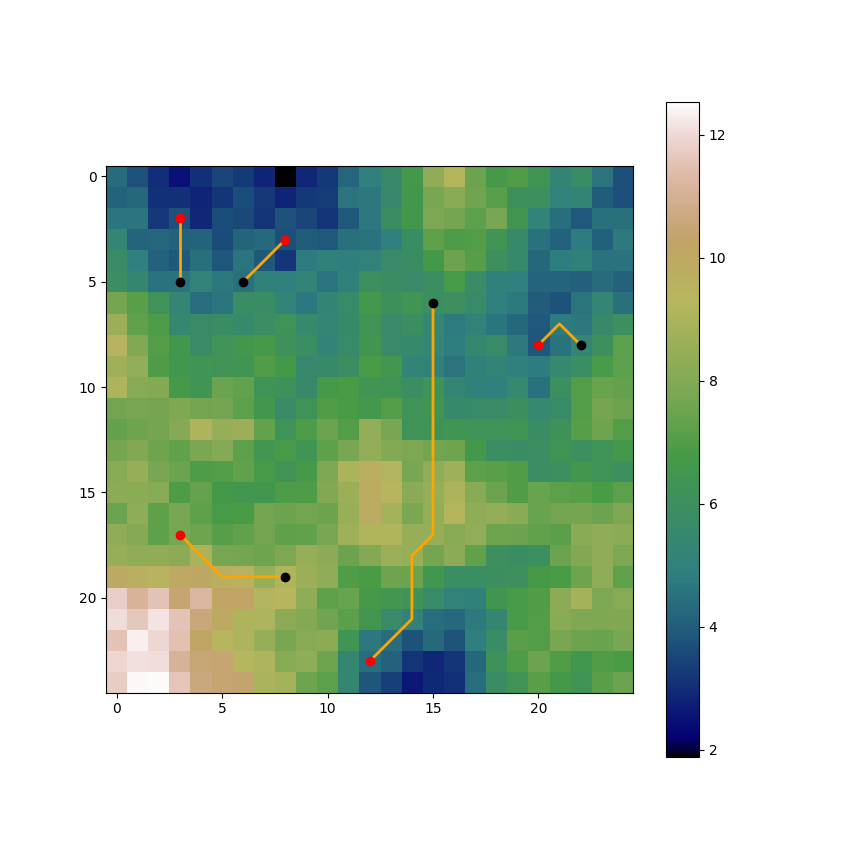
\includegraphics[width = 1.0\columnwidth]{data/mean_paths/25x25/5.png}
			\caption*{5 роботов}
			\end{subfigure}
			&
			\begin{subfigure}{0.5\linewidth}
				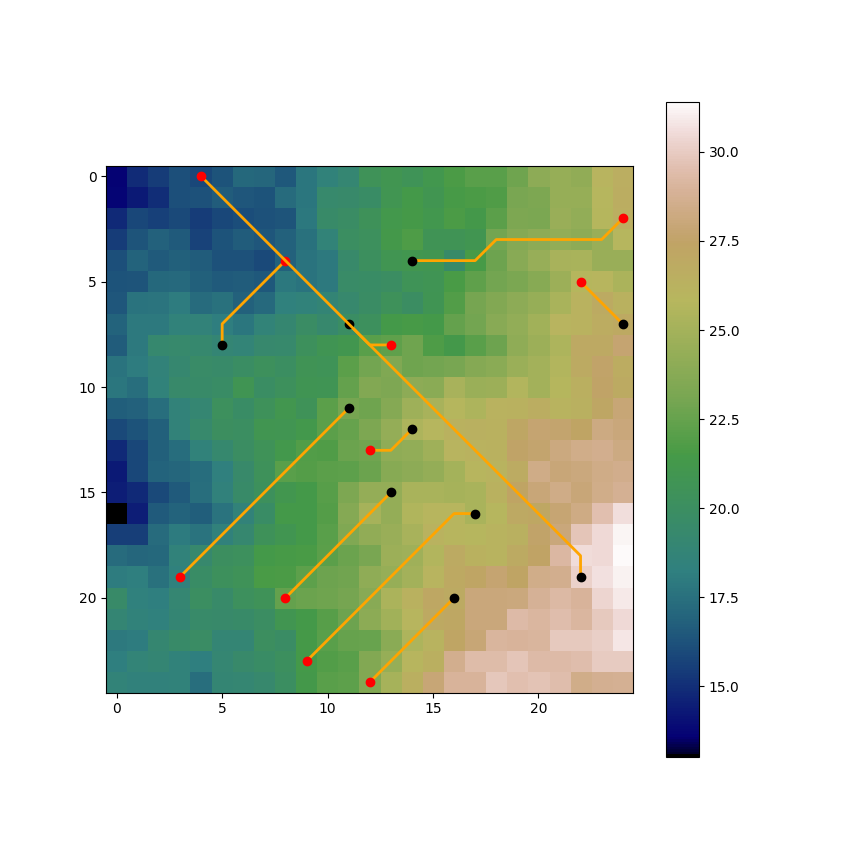
\includegraphics[width = 1.0\columnwidth]{data/mean_paths/25x25/10.png}
			\caption*{10 роботов}
			\end{subfigure}
			\\
            \begin{subfigure}{0.5\linewidth}
				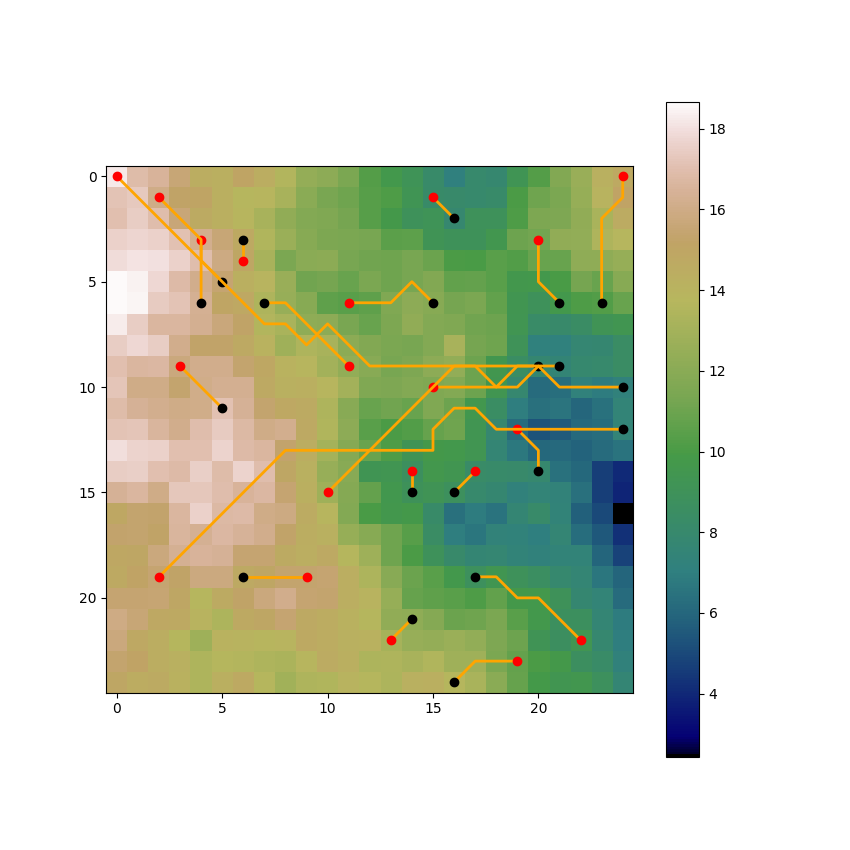
\includegraphics[width = 1.0\columnwidth]{data/mean_paths/25x25/20.png}
			\caption*{20 роботов}
			\end{subfigure}
			&
			\begin{subfigure}{0.5\linewidth}
				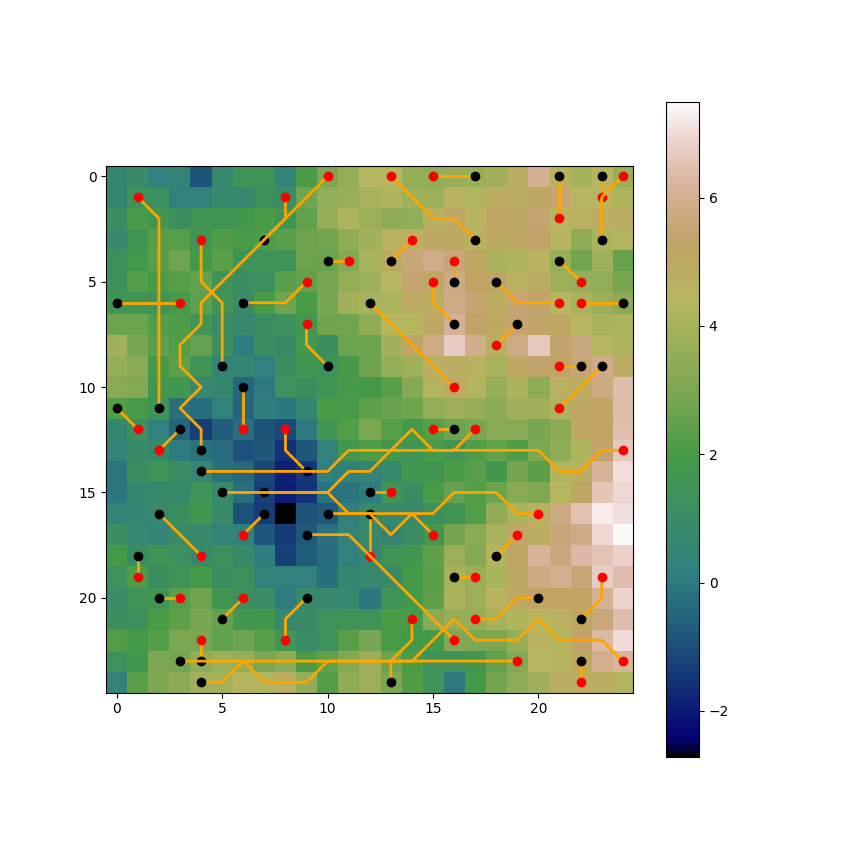
\includegraphics[width = 1.0\columnwidth]{data/mean_paths/25x25/50.png}
			\caption*{50 роботов}
			\end{subfigure}
        \end{tabular}
        \caption*{Размер карты: 25x25}
	\end{table}

	\begin{table}[H]
		\begin{tabular}{c c}
			\begin{subfigure}{0.5\linewidth}
				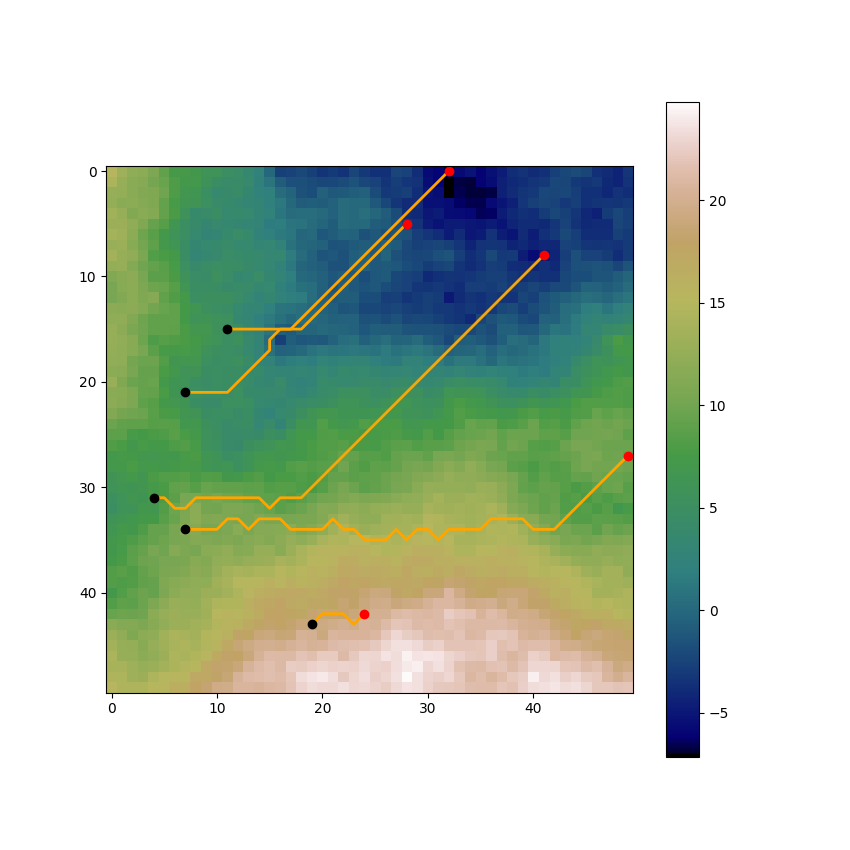
\includegraphics[width = 1.0\columnwidth]{data/mean_paths/50x50/5.png}
			\caption*{5 роботов}
			\end{subfigure}
			&
			\begin{subfigure}{0.5\linewidth}
				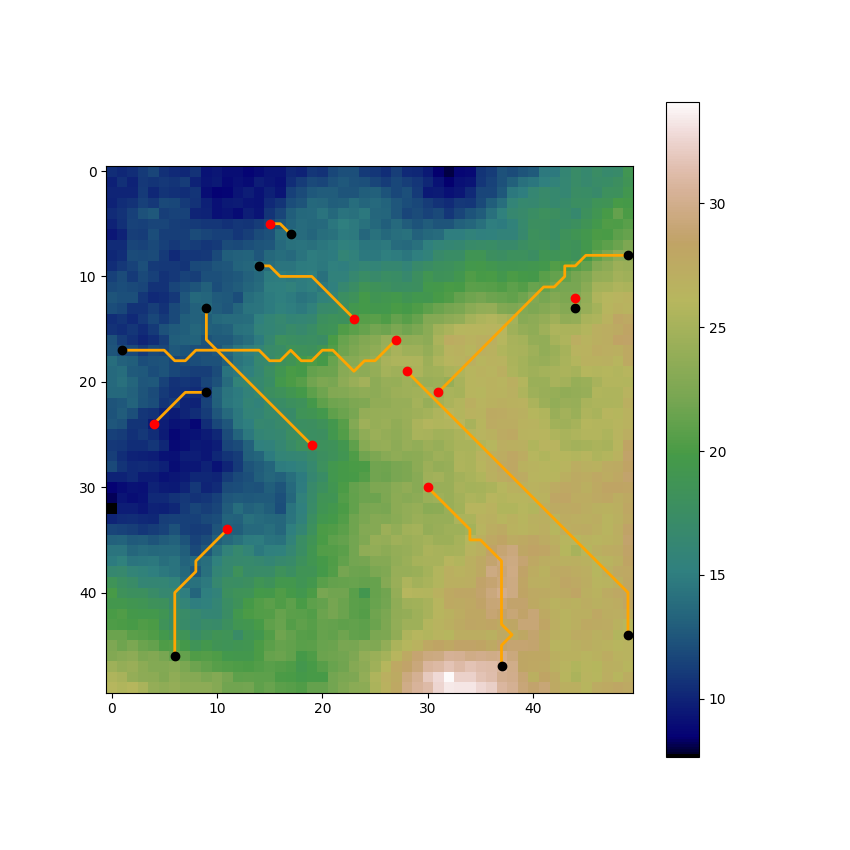
\includegraphics[width = 1.0\columnwidth]{data/mean_paths/50x50/10.png}
			\caption*{10 роботов}
			\end{subfigure}
			\\
            \begin{subfigure}{0.5\linewidth}
				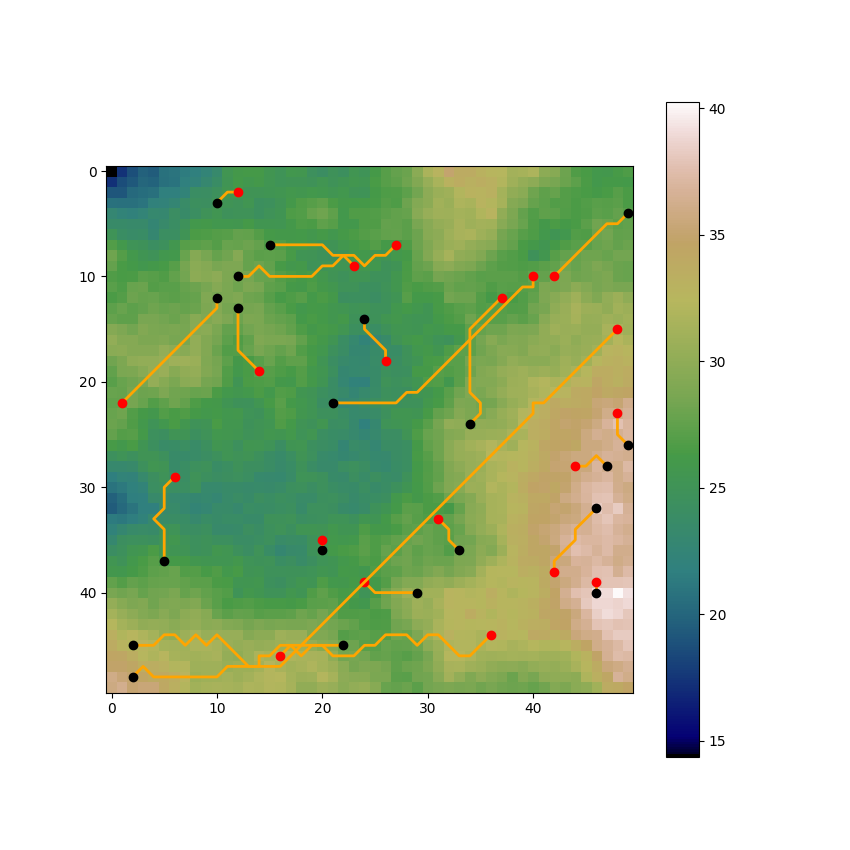
\includegraphics[width = 1.0\columnwidth]{data/mean_paths/50x50/20.png}
			\caption*{20 роботов}
			\end{subfigure}
			&
			\begin{subfigure}{0.5\linewidth}
				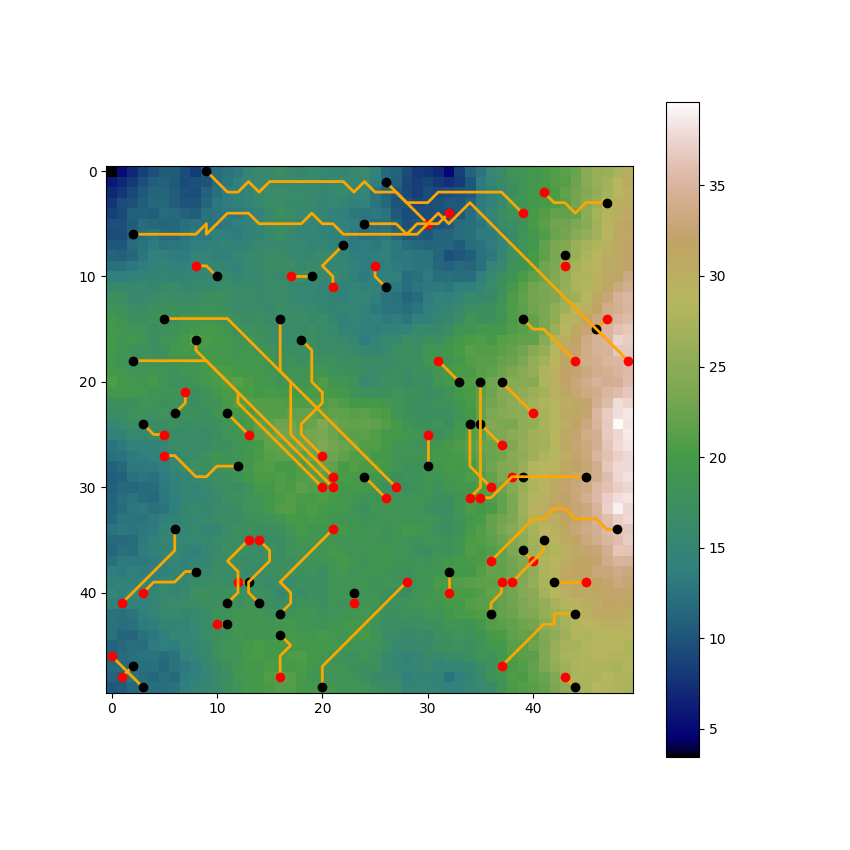
\includegraphics[width = 1.0\columnwidth]{data/mean_paths/50x50/50.png}
			\caption*{50 роботов}
			\end{subfigure}
        \end{tabular}
        \caption*{Размер карты: 50x50}
	\end{table}

	\begin{table}[H]
		\begin{tabular}{c c}
			\begin{subfigure}{0.5\linewidth}
				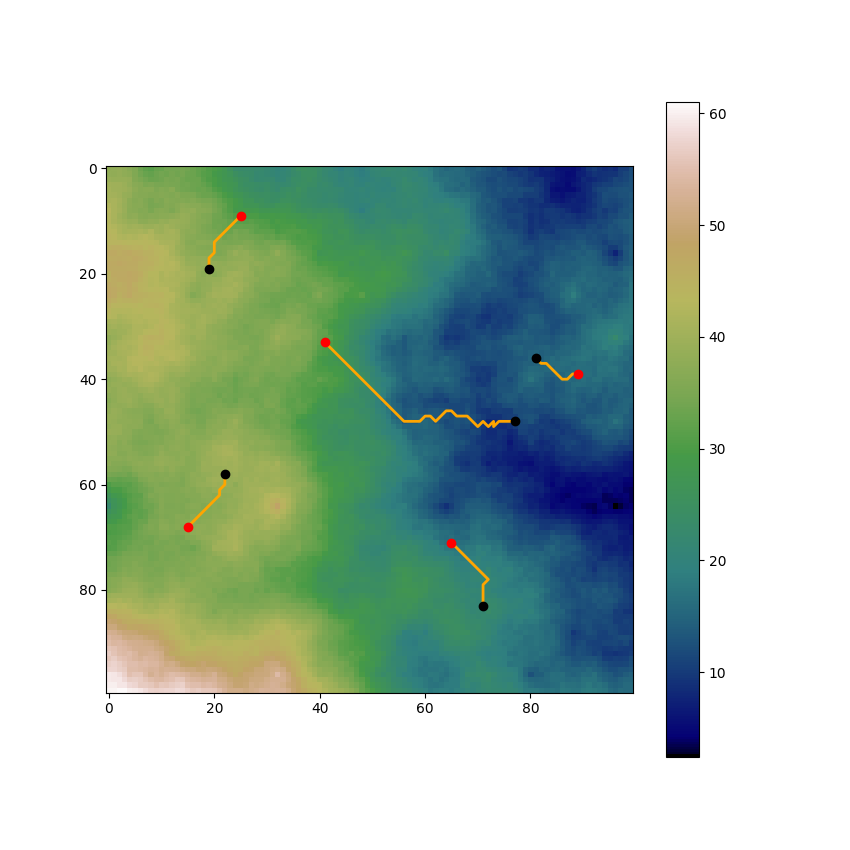
\includegraphics[width = 1.0\columnwidth]{data/mean_paths/100x100/5.png}
			\caption*{5 роботов}
			\end{subfigure}
			&
			\begin{subfigure}{0.5\linewidth}
				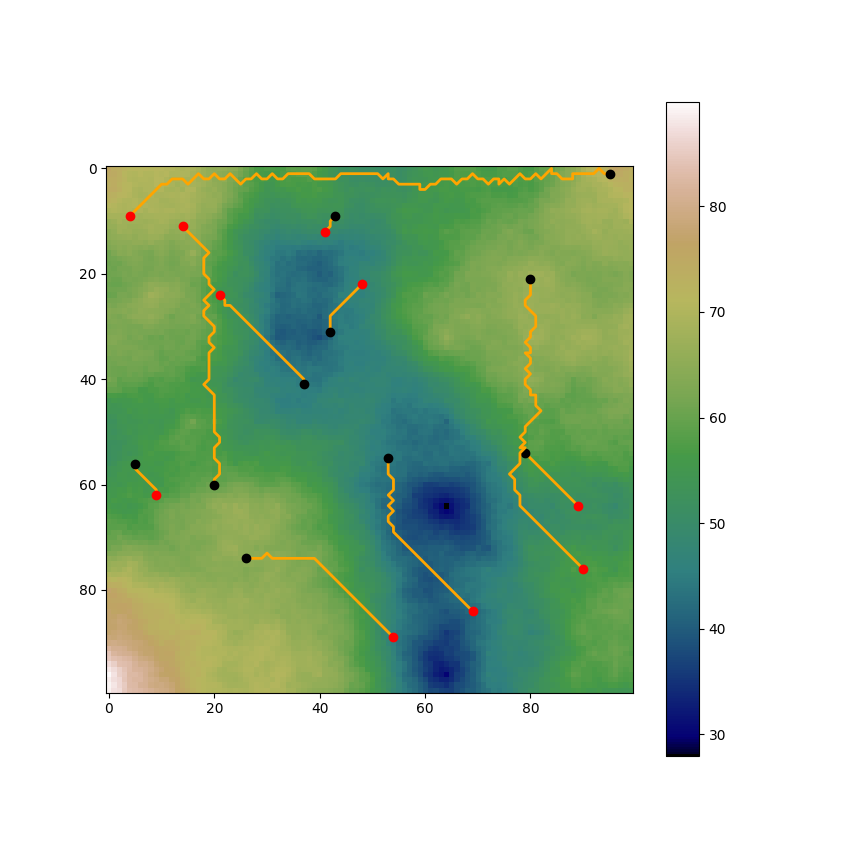
\includegraphics[width = 1.0\columnwidth]{data/mean_paths/100x100/10.png}
			\caption*{10 роботов}
			\end{subfigure}
			\\
            \begin{subfigure}{0.5\linewidth}
				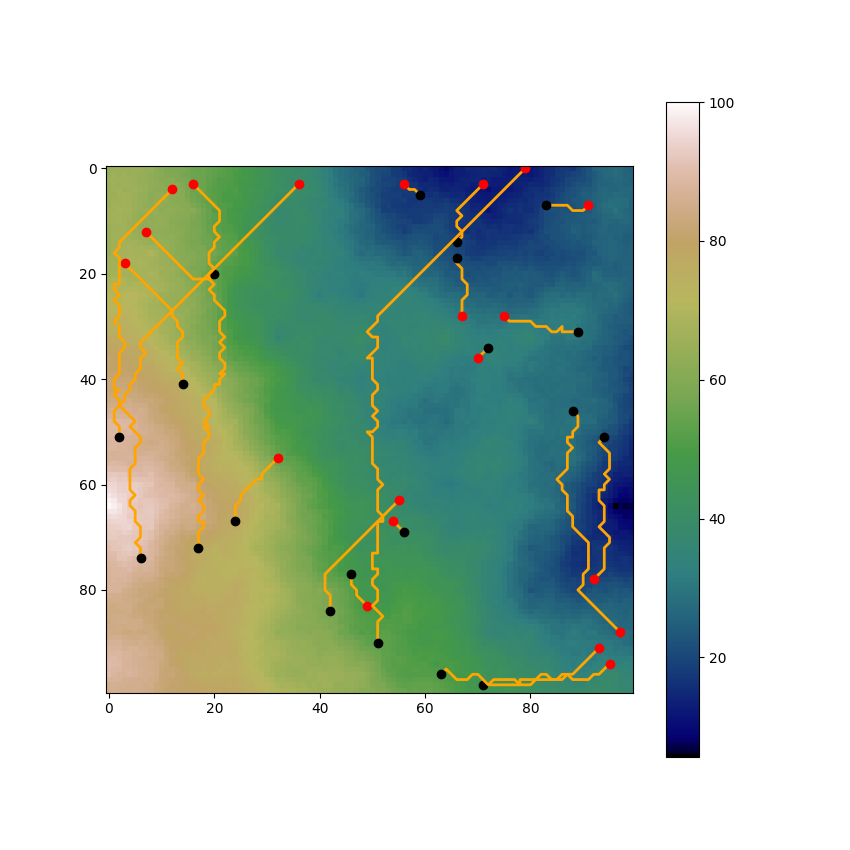
\includegraphics[width = 1.0\columnwidth]{data/mean_paths/100x100/20.png}
			\caption*{20 роботов}
			\end{subfigure}
			&
			\begin{subfigure}{0.5\linewidth}
				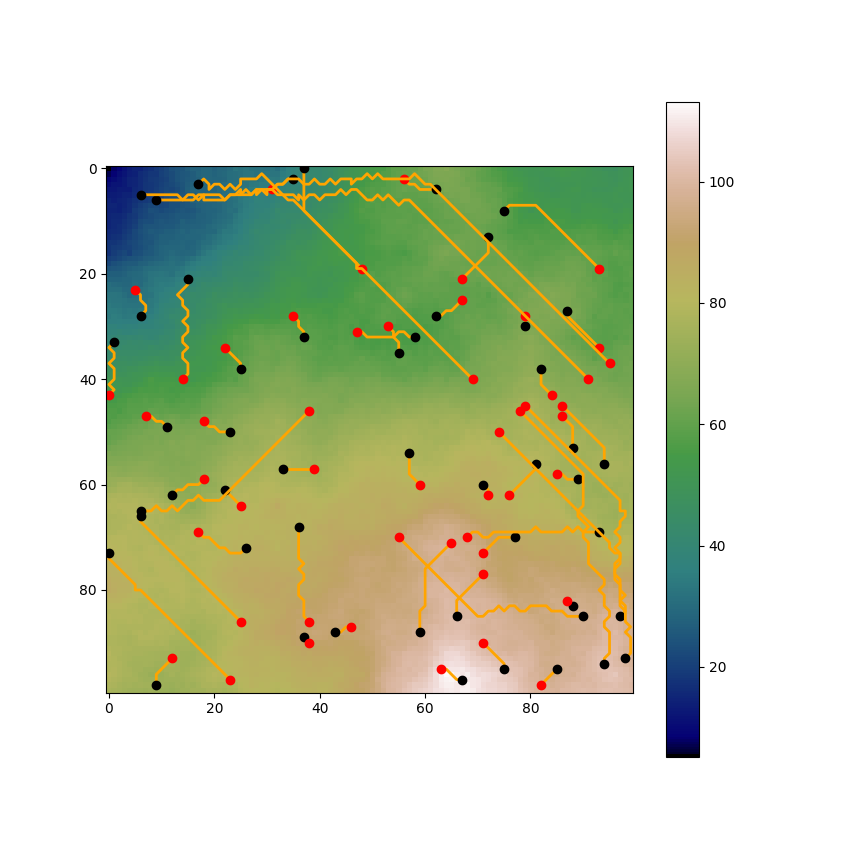
\includegraphics[width = 1.0\columnwidth]{data/mean_paths/100x100/50.png}
			\caption*{50 роботов}
			\end{subfigure}
        \end{tabular}
        \caption*{Размер карты: 100x100}
	\end{table}

	\begin{table}[H]
		\begin{tabular}{c c}
			\begin{subfigure}{0.5\linewidth}
				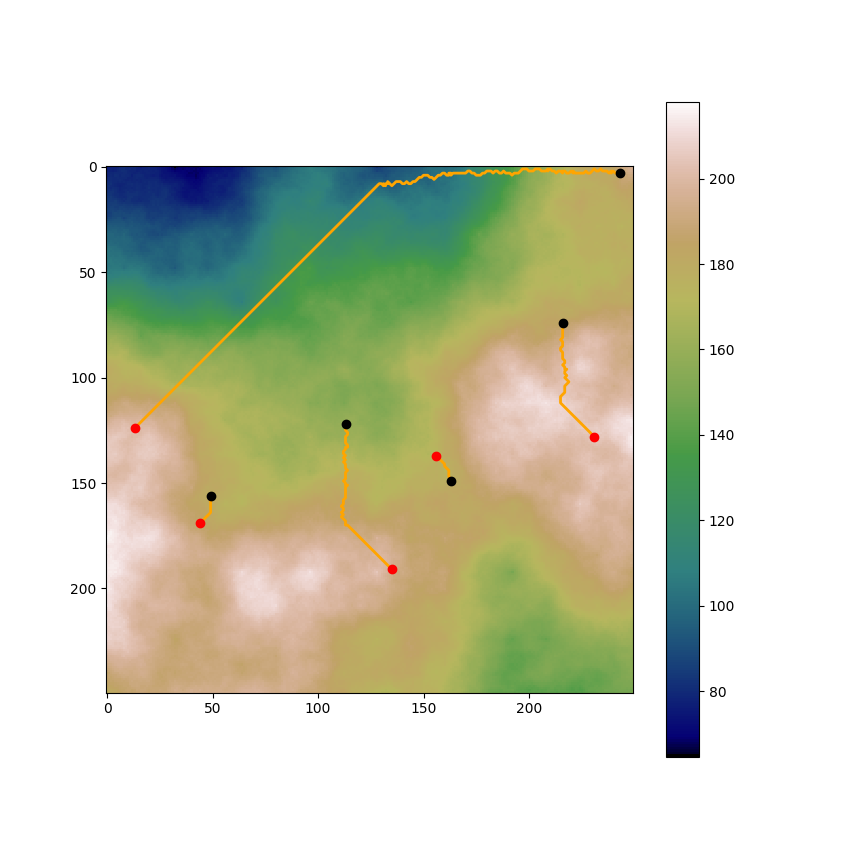
\includegraphics[width = 1.0\columnwidth]{data/mean_paths/250x250/5.png}
			\caption*{5 роботов}
			\end{subfigure}
			&
			\begin{subfigure}{0.5\linewidth}
				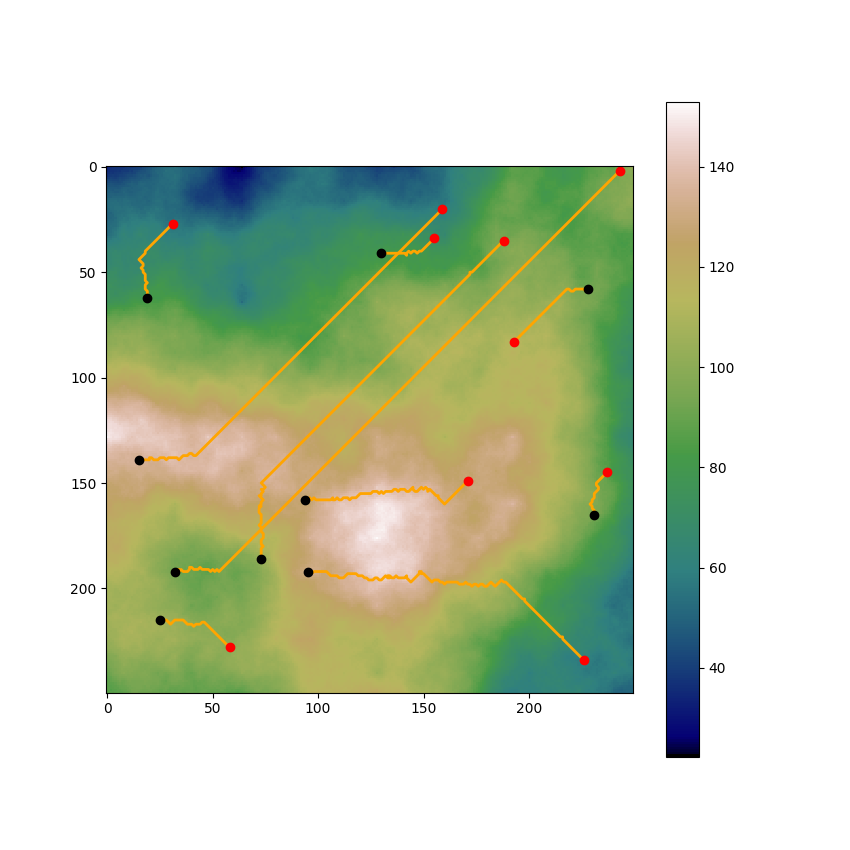
\includegraphics[width = 1.0\columnwidth]{data/mean_paths/250x250/10.png}
			\caption*{10 роботов}
			\end{subfigure}
			\\
            \begin{subfigure}{0.5\linewidth}
				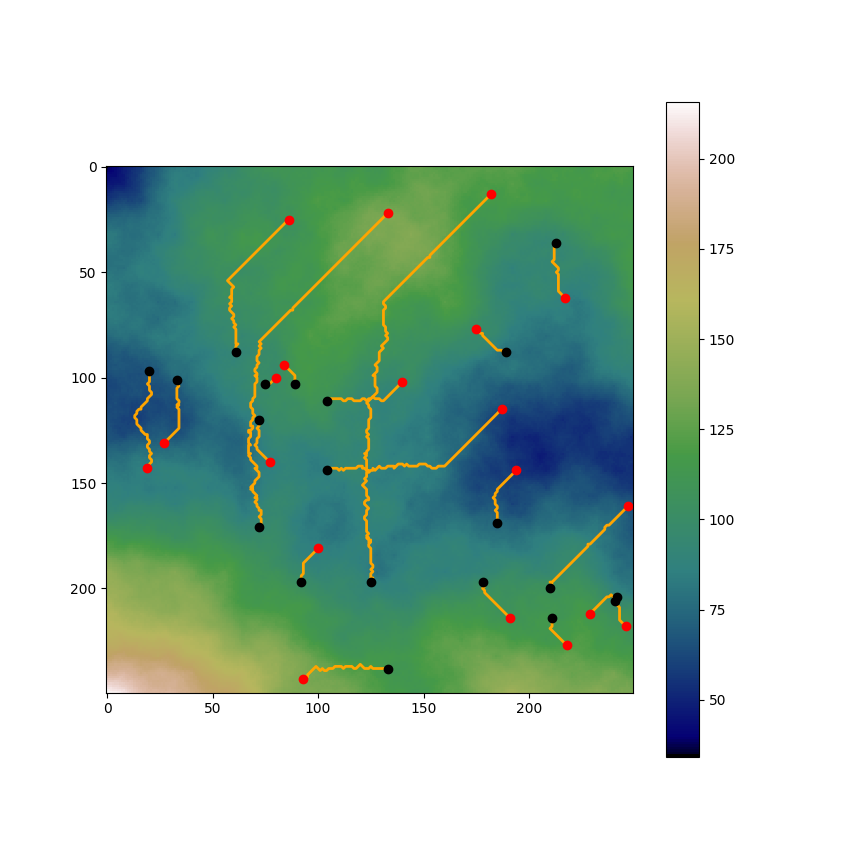
\includegraphics[width = 1.0\columnwidth]{data/mean_paths/250x250/20.png}
			\caption*{20 роботов}
			\end{subfigure}
			&
			\begin{subfigure}{0.5\linewidth}
				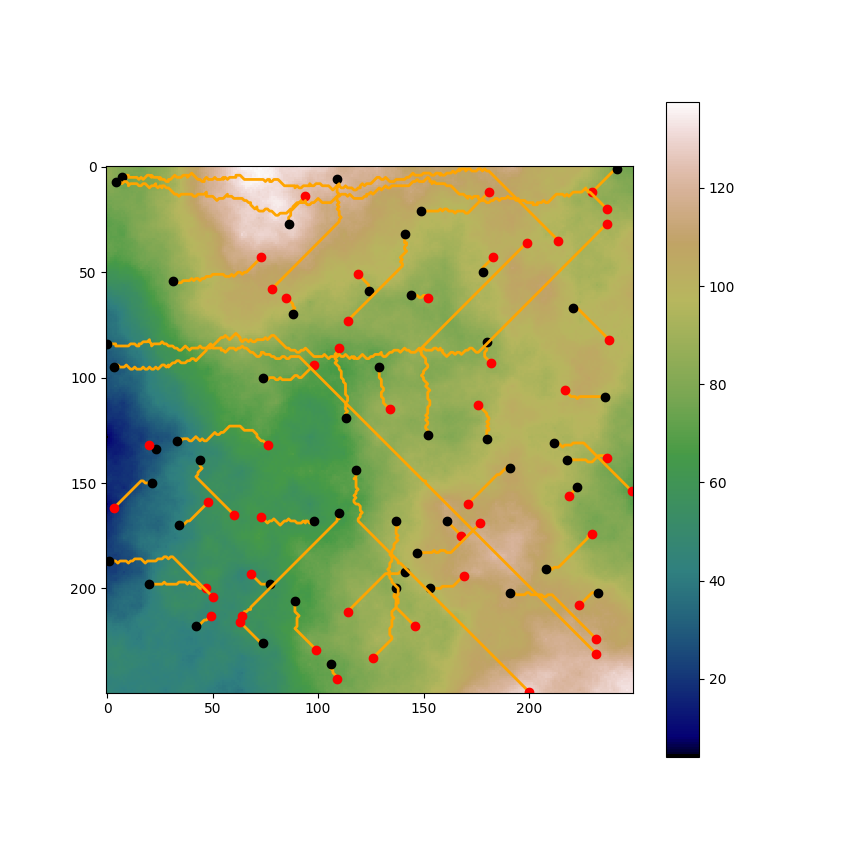
\includegraphics[width = 1.0\columnwidth]{data/mean_paths/250x250/50.png}
			\caption*{50 роботов}
			\end{subfigure}
        \end{tabular}
        \caption*{Размер карты: 250x250}
	\end{table}

	\begin{table}[H]
		\begin{tabular}{c c}
			\begin{subfigure}{0.5\linewidth}
				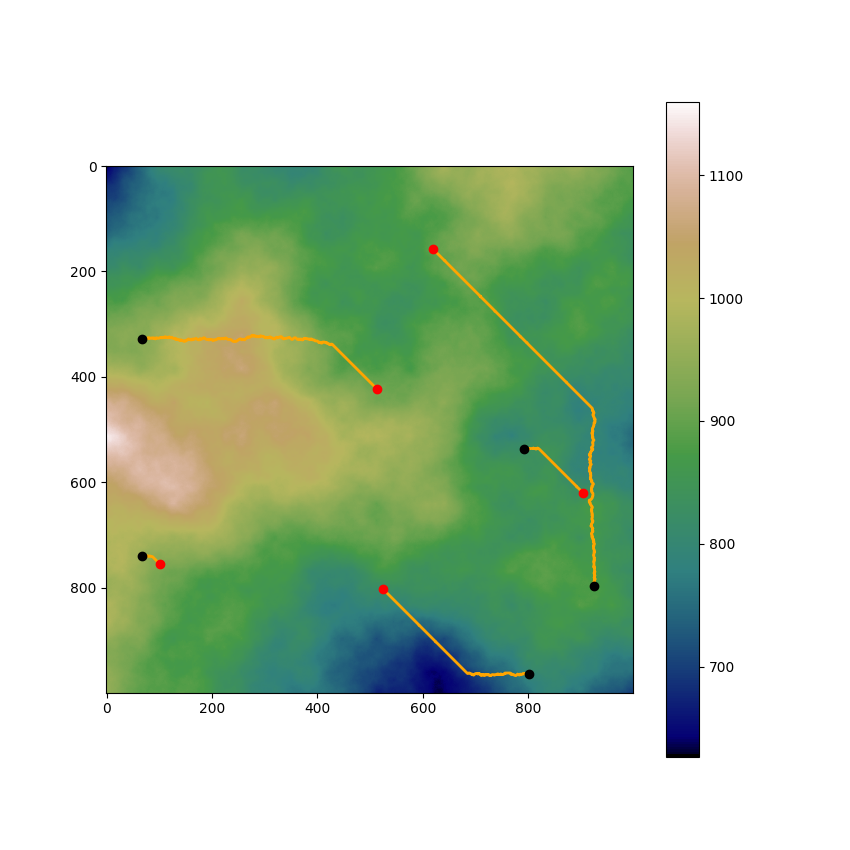
\includegraphics[width = 1.0\columnwidth]{data/mean_paths/1000x1000/5.png}
			\caption*{5 роботов}
			\end{subfigure}
			&
			\begin{subfigure}{0.5\linewidth}
				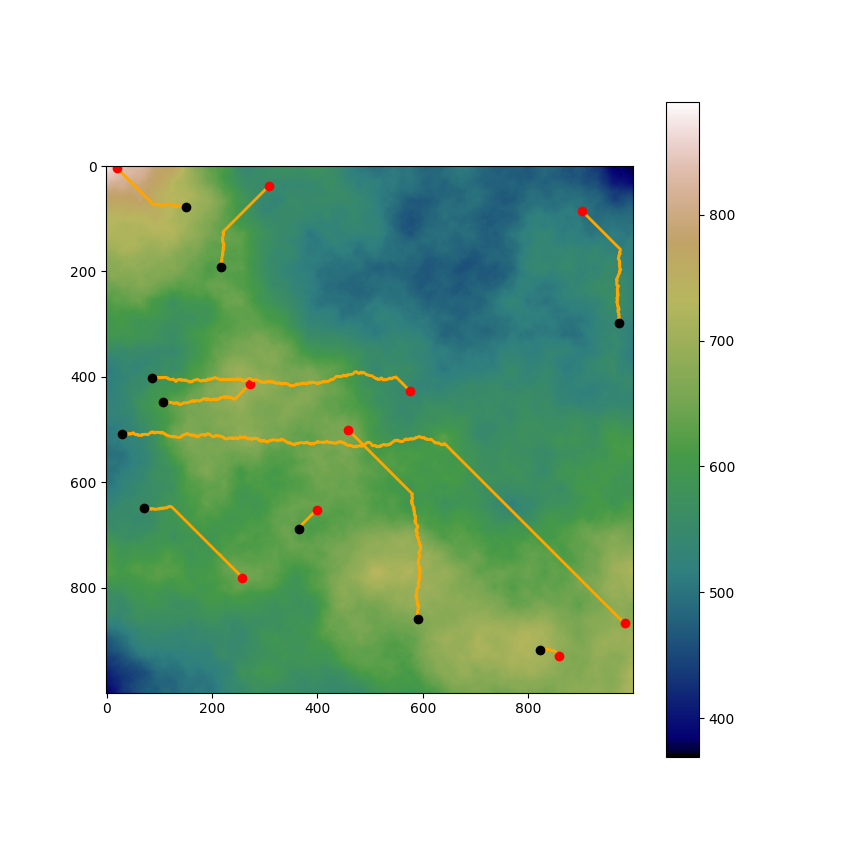
\includegraphics[width = 1.0\columnwidth]{data/mean_paths/1000x1000/10.png}
			\caption*{10 роботов}
			\end{subfigure}
			\\
            \begin{subfigure}{0.5\linewidth}
				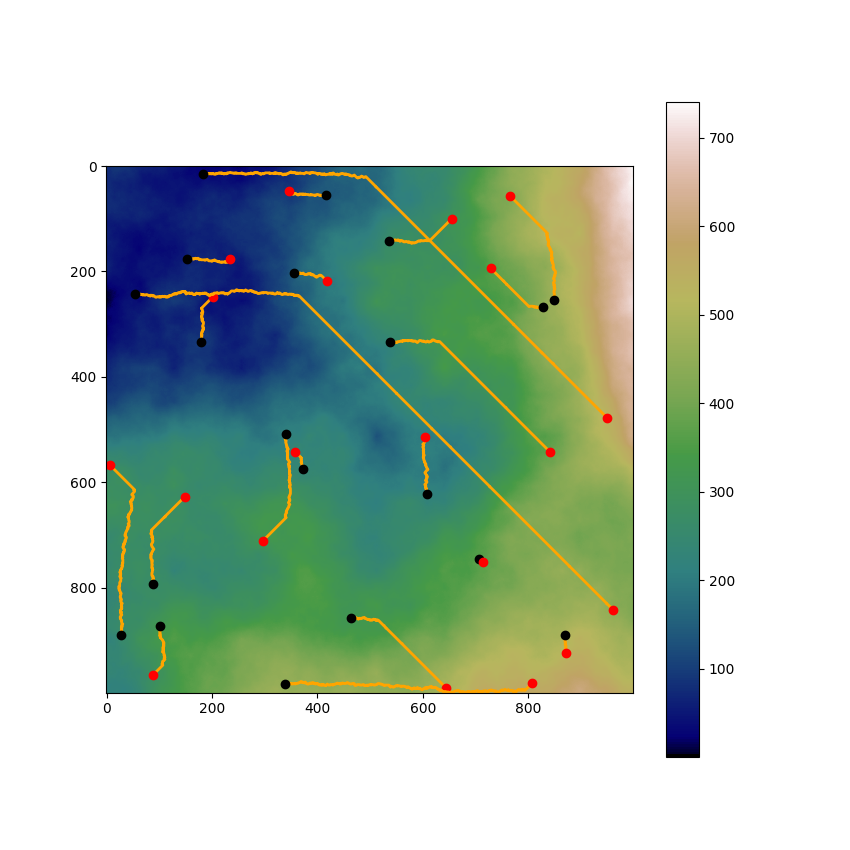
\includegraphics[width = 1.0\columnwidth]{data/mean_paths/1000x1000/20.png}
			\caption*{20 роботов}
			\end{subfigure}
			&
			\begin{subfigure}{0.5\linewidth}
				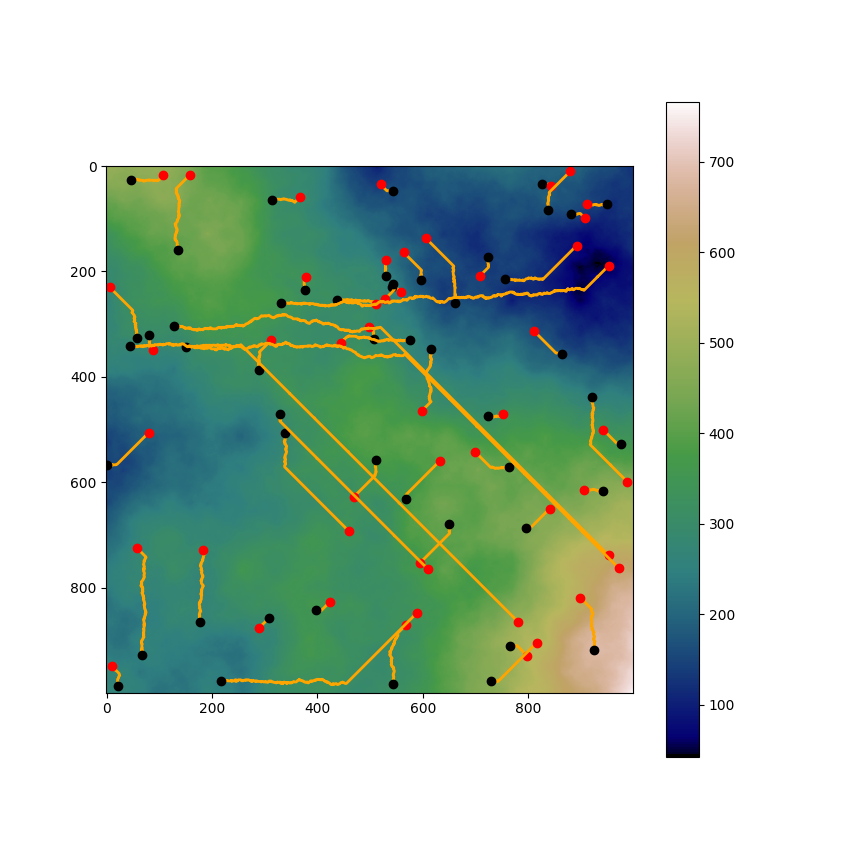
\includegraphics[width = 1.0\columnwidth]{data/mean_paths/1000x1000/50.png}
			\caption*{50 роботов}
			\end{subfigure}
        \end{tabular}
        \caption*{Размер карты: 1000x1000}
	\end{table}

\end{document}
